\documentclass[a4paper,12pt]{report}

\usepackage{polski}
\usepackage[polish]{babel}
\usepackage[utf8]{inputenc}
\usepackage{indentfirst}
\usepackage[hidelinks]{hyperref}
\usepackage[table]{xcolor}
\usepackage{tabularx}
\usepackage[backend=biber,sorting=ynt]{biblatex}
\addbibresource{bibliography.bib}

\usepackage{caption}
\usepackage[newfloat]{minted}
\captionsetup[listing]{position=top}

\usepackage{csquotes}
\DeclareQuoteStyle{polish}
  {\itshape\quotedblbase}
  {\itshape\textquotedblright}
  [0.05em]
  {\guillemotright}
  {\guillemotleft}
\setquotestyle{polish}  

\usepackage{graphicx}
\graphicspath{ {images/} }

\usepackage{pifont}
\newcommand{\checkmark}{\ding{51}}

\usepackage{threeparttable}
\usepackage{tabu}
\usepackage{xpatch}
\makeatletter
\chardef\TPT@@@asteriskcatcode=\catcode`*
\catcode`*=11
\xpatchcmd{\threeparttable}
  {\TPT@hookin{tabular}}
  {\TPT@hookin{tabular}\TPT@hookin{tabu}}
  {}{}
\catcode`*=\TPT@@@asteriskcatcode
\makeatother
\usepackage{array}

\newcommand\Thickvrule[1]{%
  \multicolumn{1}{!{\vrule width 2pt}c!{\vrule width 2pt}}{#1}%
}

\usepackage{tikz}
\usepackage{amsmath}
\usepackage{amsthm}
\newtheorem{theorem}{\normalfont\scshape Twierdzenie}

\usepackage{caption}
\usepackage[bottom]{footmisc}

\usepackage{chemfig}
\setatomsep{2em}

\usepackage{booktabs}

\begin{document}
\definecolor{light-gray}{gray}{0.95}
\definecolor{lighter-gray}{gray}{0.65}
\tikzset{every node/.style={fill,circle,scale=0.5,font=\huge}}
\begin{titlepage}
\centering
\textbf{\Large Uniwersytet Jagielloński w Krakowie}\par
\vspace{0.2cm}
{\Large Wydział Fizyki, Astronomii i Informatyki Stosowanej}\par
\vfill
\textbf{\Large Łukasz Kostrzewa}\par
\vspace{0.2cm}
{\small Nr albumu: 1080514\par}
\vspace{1.5cm}
\textbf{\huge Wizualizacja, edycja i~przetwarzanie grafów on-line}\par
\vspace{1cm}
Praca magisterska\par
na kierunku Informatyka stosowana\par
\vfill
\begin{flushright}
Praca wykonana pod kierunkiem \par
dr hab. Barbary Strug\par
Zakład Projektowania i Grafiki Komputerowej\par
\end{flushright}
\vspace{1cm}
Kraków 2016\par
\end{titlepage}
\noindent {\large \textbf{Oświadczenie autora pracy}}\\

\noindent Świadom odpowiedzialności prawnej oświadczam, że niniejsza praca dyplomowa została napisana przeze mnie samodzielnie i nie zawiera treści uzyskanych w sposób niezgodny z obowiązującymi przepisami.

\vspace{0.3cm}
\noindent Oświadczam również, że przedstawiona praca nie była wcześniej przedmiotem procedur związanych z uzyskaniem tytułu zawodowego w wyższej uczelni.
\vspace{2cm}

\noindent Kraków, dnia \hfill Podpis autora pracy

\vspace{4cm}

\noindent {\large \textbf{Oświadczenie kierującego pracą}}\\

\noindent Potwierdzam, że niniejsza praca została przygotowana pod moim kierunkiem i kwalifikuje się do przedstawienia jej w postępowaniu o nadanie tytułu zawodowego.
\vspace{2cm}

\noindent Kraków, dnia \hfill Podpis kierującego pracą
\thispagestyle{empty}


\tableofcontents
\thispagestyle{empty}

\chapter*{Wstęp}
\addcontentsline{toc}{chapter}{Wstęp}

\blockquote[L. Euler]{\enquote{This question is so banal, but seemed to me worthy of attention in that [neither] geometry, nor algebra, nor even the art of counting was sufficient to solve it.}}

tbc

\thispagestyle{empty}

\chapter{Wprowadzenie}
\section{Czym są grafy}
\section{Zastosowania grafów}
\chapter{Istniejące rozwiązania}

W tym rozdziale przedstawię istniejące aplikacje internetowe \cite{mathex} i desktopowe służące do tworzenia i wizualizacji grafów. Tabela \ref{tab:app-comparison} zawiera porównanie funkcjonalności opisywanych darmowych aplikacji internetowych oraz aplikacji \emph{Graphy} -- tworzonej w ramach tej pracy. 

Głównie skupię się na aplikacjach internetowych ze względu na związek z tematem mojej pracy. 

\section{Aplikacje internetowe}

\subsection*{Graph Creator}
\bigskip
\noindent\begin{tabularx}{\textwidth}{r|X|}
\cline{2-2}
  Adres URL & http://illuminations.nctm.org/Activity.aspx?id=3550 \\ 
\cline{2-2}
 Autor & National Council of Teachers of Mathematics \\ 
\cline{2-2}
 Licencja & Darmowa\\  
\cline{2-2}
\end{tabularx} 
\bigskip

Aplikacja pozwala tworzyć grafy skierowane i nieskierowane. Posiada możliwość kolorowania wierzchołków, wyrównania ich do siatki oraz ustawienia wag na krawędziach i etykiet w wierzchołkach. Ponadto użytkownik może wyświetlić stopnie wierzchołków oraz wyginać krawędzie. Dodatkową funkcjonalnością jest możliwość zaznaczenia kilku wierzchołków na raz. 

\textit{Graph Creator} nie daje możliwości eksportowania i importowania grafów. Nie można również przesuwać widoku ani oddalać oraz przybliżać grafu. Aplikacja posiada ograniczenie liczby wierzchołków -- maksymalna dozwolona ilość to 52 wierzchołki.

\begin{figure}[H]
\centering
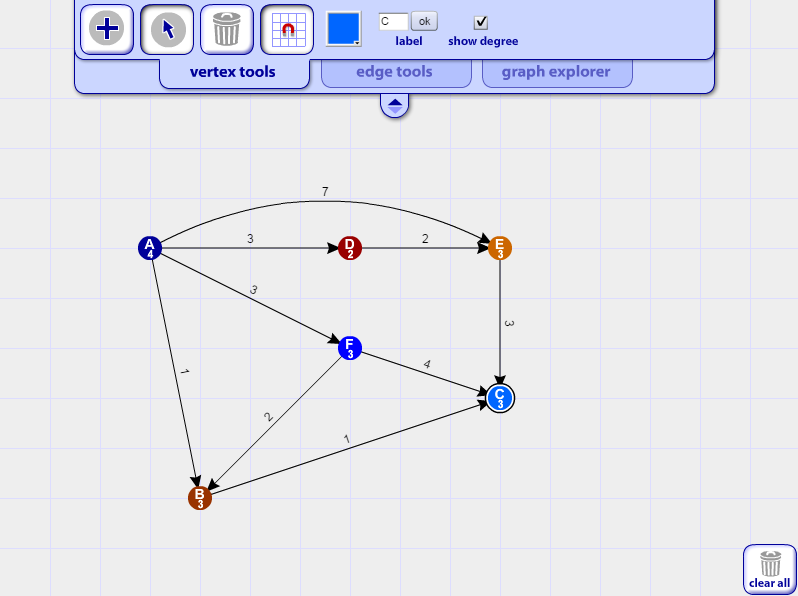
\includegraphics[width=\textwidth]{graph-creator.png}
\caption{Zrzut ekranu z aplikacji Graph Creator}
\end{figure}

\subsection*{Graph Online}
\bigskip
\noindent\begin{tabularx}{\textwidth}{r|X|}
\cline{2-2}
  Adres URL & http://graphonline.ru/en/ \\ 
\cline{2-2}
 Autor & Unick-soft \\ 
\cline{2-2}
 Licencja & Darmowa\\  
\cline{2-2}
\end{tabularx} 
\bigskip

Aplikacja również daje możliwość stworzenia grafów zarówno skierowanych jak i nieskierowanych. Podobnie jak poprzednia aplikacja pozwala na zmianę etykiet wierzchołków, nadanie wag krawędziom oraz na wyświetlenie stopnia wierzchołków. Ponadto użytkownik ma możliwość przesuwania widoku oraz jego przybliżania i oddalania. Dodatkowo \textit{Graph Online} pozwala zapisać graf jako macierz sąsiedztwa lub incydencji oraz wczytać graf zapisany w takiej postaci. Użytkownik może również zapisać graf na serwerze -- po zapisaniu wyświetlany jest ogólnodostępny adres URL do grafu. Ciekawą funkcjonalnością jest eksport grafu do obrazka (plik \texttt{PNG}).

\textit{Graph Online} posiada możliwość wykonania podstawowych algorytmów na grafie, takich jak: znajdowanie najkrótszej ścieżki pomiędzy dwoma wierzchołkami, znajdowanie cyklu Eulera, znajdowanie spójnych składowych, znajdowanie minimalnego drzewa rozpinającego.  

W przeciwieństwie do poprzedniej aplikacji nie mamy możliwości kolorowania wierzchołków, zaznaczania kilku wierzchołków na raz oraz wyginania krawędzi. Maksymalna dozwolona ilość wierzchołków to 299. 

\begin{figure}[H]
\centering
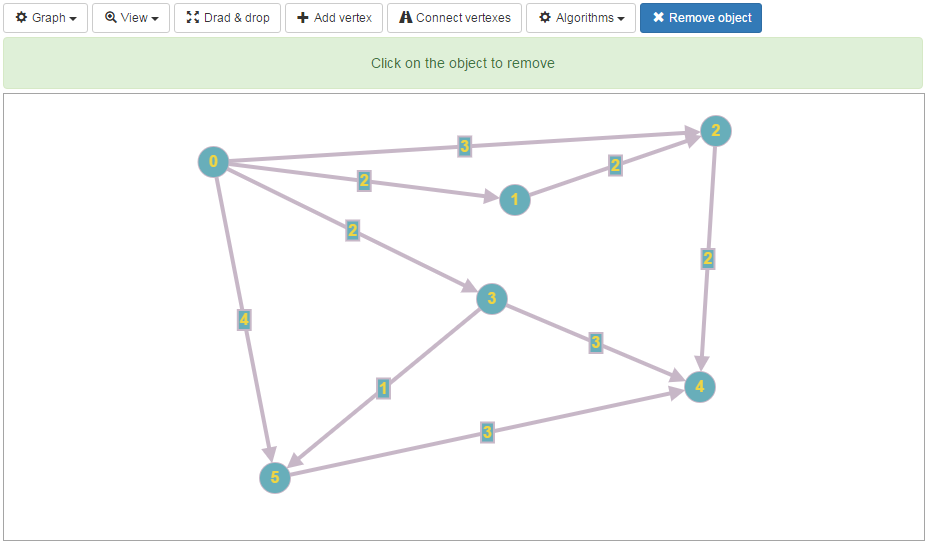
\includegraphics[width=\textwidth]{graph-online.png}
\caption{Zrzut ekranu z aplikacji Graph Online}
\end{figure}

\subsection*{GraphJS}
\bigskip
\noindent\begin{tabularx}{\textwidth}{r|X|}
\cline{2-2}
  Adres URL & https://dl.dropboxusercontent.com/u/4189520/GraphJS/ graphjs.html \\ 
\cline{2-2} 
 Autor & David Kofoed Wind \\ 
\cline{2-2}
 Licencja & Darmowa\\  
\cline{2-2}
\end{tabularx}
\bigskip

Aplikacja pozwala na tworzenie grafów nieskierowanych. Podobnie jak w poprzednich aplikacjach możemy nadawać etykiety wierzchołkom i krawędziom. Niespotykaną funkcjonalnością jest możliwość stworzenia kilku grafów i przełączania się pomiędzy nimi oraz możliwość eksportu grafu do formatu \LaTeX (pakiet Ti\textit{k}Z). Ponadto użytkownik ma możliwość eksportu do własnego formatu \texttt{JSON} oraz importu grafu z tego formatu. Aplikacja posiada funkcjonalność zaznaczania wielu wierzchołków na raz.

W \textit{GraphJS} nie ma możliwości przesuwania widoku oraz przybliżania i~oddalania grafu. Nie ma również możliwości kolorowania wierzchołków oraz wyginania krawędzi. Aplikacja zdaje się nie mieć limitu na liczbę wierzchołków -- udało się wczytać graf $C_{1000}$ jednakże dodanie kolejnego wierzchołka zajmuje około 10 sekund.

\begin{figure}[H]
\centering
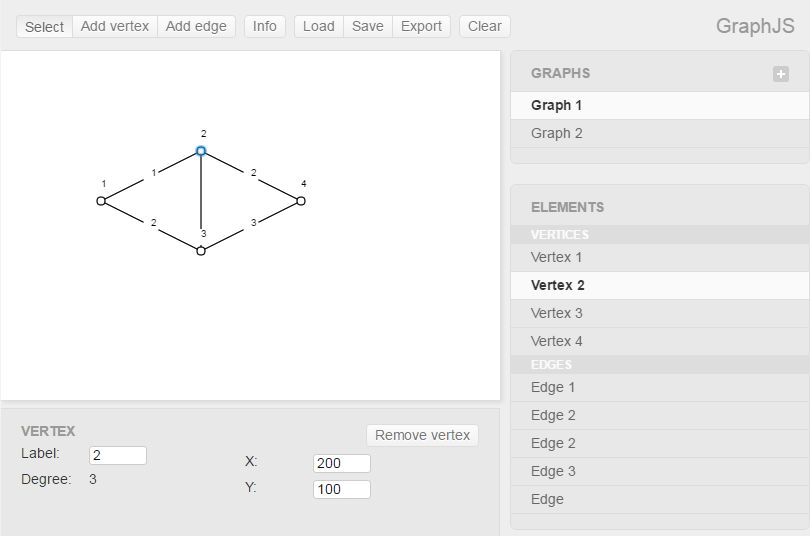
\includegraphics[width=\textwidth]{graphjs.png}
\caption{Zrzut ekranu z aplikacji GraphJS}
\end{figure}


\subsection*{Graphrel}
\bigskip
\noindent\begin{tabularx}{\textwidth}{r|X|}
\cline{2-2}
  Adres URL & https://yiboyang.github.io/graphrel/ \\ 
\cline{2-2} 
 Autor & Yibo Yang \\
\cline{2-2}
 Licencja & Darmowa\\  
\cline{2-2}
\end{tabularx} 
\bigskip

Aplikacja daje możliwość tworzenia grafów skierowanych. W przeciwieństwie do poprzednio opisywanych aplikacji posiada układ kierowany siłą (ang. \textit{force-directed layout}), choć istnieje również opcja samodzielnego rozstawienia wierzchołków -- poprzez przytrzymanie klawisza \texttt{Ctrl}. Użytkownik może zaimportować graf z formatu stworzonego przez aplikację (tablice list sąsiedztwa dla każdego wierzchołka). Bardzo przydatną i niespotykaną funkcjonalnością jest możliwość cofania oraz ponawiania ostatnich akcji. 

W \textit{Graphrel} nie możemy nadawać własnych etykiet na krawędziach ani w wierzchołkach, nie możemy przesuwać widoku ani zmieniać przybliżenia grafu. Nie ma również możliwości wyginania krawędzi, zaznaczania kliku wierzchołków na raz oraz kolorowania wierzchołków. Do aplikacji udało się wczytać graf $C_{100}$, przy próbie wczytania $C_{101}$ pojawia się informacja o niepoprawnym formacie.

\begin{figure}[H]
\centering
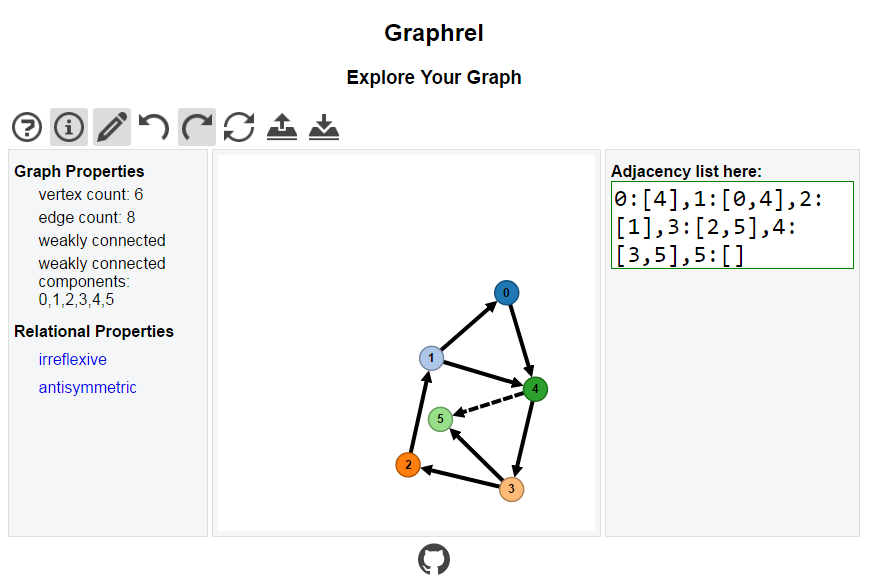
\includegraphics[width=\textwidth]{graphrel.png}
\caption{Zrzut ekranu z aplikacji Graphrel}
\end{figure}

\subsection*{VisuAlgo}
\bigskip
\noindent\begin{tabularx}{\textwidth}{r|X|}
\cline{2-2}
  Adres URL & https://visualgo.net/en/ \\ 
\cline{2-2} 
 Autor & Dr Steven Halim \\ 
\cline{2-2}
 Licencja & Darmowa\\ 
\cline{2-2}
\end{tabularx} 
\bigskip

Aplikacja stworzona przez Dr Stevena Halima z National University of Singapore. Posiada możliwość tworzenia prostych grafów, jednak jej głównym celem nie jest tworzenie grafów, lecz wizualizacja algorytmów przez animację (nie tylko na grafach, ale również na strukturach danych). Użytkownik wraz z przebiegiem algorytmu może obserwować przebieg kodu, może zatrzymać się w dowolnym jego kroku, cofnąć się do kroku poprzedniego albo przejść do następnego.

\begin{figure}[H]
\centering
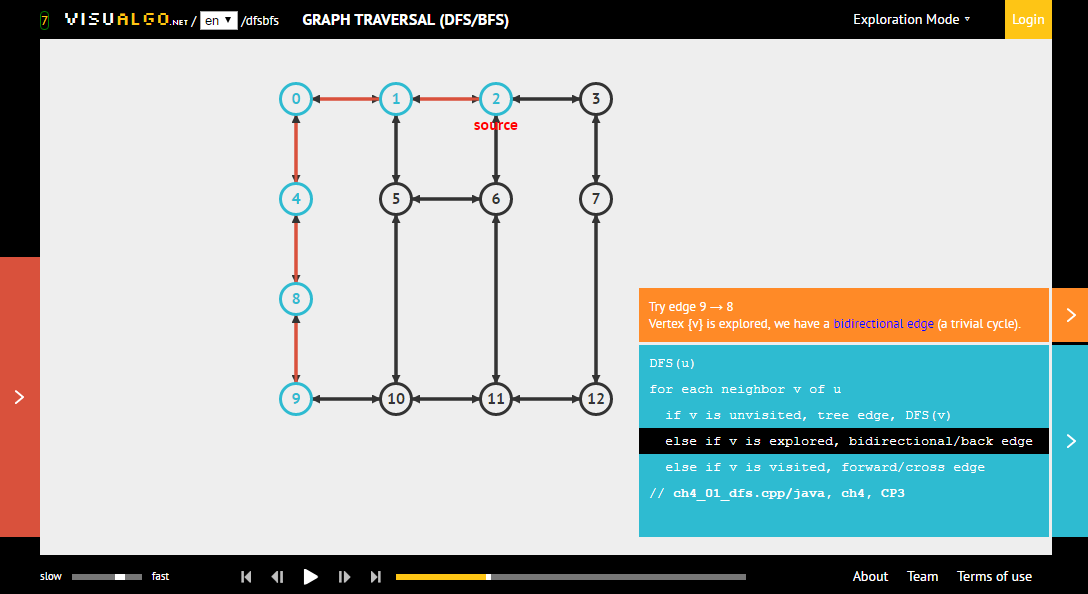
\includegraphics[width=\textwidth]{visualgo.png}
\caption{Zrzut ekranu z aplikacji VisuAlgo}
\end{figure}

\subsection*{yEd Live}
\bigskip
\noindent\begin{tabularx}{\textwidth}{r|X|}
\cline{2-2}
  Adres URL & https://www.yworks.com/yed-live/ \\ 
\cline{2-2} 
 Autor & yWorks\\ 
\cline{2-2}
 Licencja & Darmowa i płatna\\ 
\cline{2-2}
\end{tabularx}
\bigskip

Internetowa wersja aplikacji yEd stworzona przez firmę yWorks. Pozwala na tworzenie dowolnych grafów (skierowanych, nieskierowanych). W aplikacji istnieje możliwość nadawania etykiet wierzchołkom i krawędziom. Twórcy dostarczyli również możliwość kolorowania wierzchołków, zmiany ich kształtu, a nawet ustawiania obrazków w wierzchołkach. Użytkownik może też dowolnie wyginać krawędzie. Niespotykaną funkcjonalnością jest możliwość grupowania wierzchołków. 

Jeśli chodzi o wyświetlanie grafu, to \textit{yEd Live} dostarcza mały podgląd grafu, dzięki któremu możemy przesuwać graf. Istnieje też opcja przybliżania i oddalania grafu. Dodatkową funkcjonalnością jest zmiana układu wierzchołków (m.in. na układ hierarchiczny, ortogonalny czy kołowy) oraz wyszukiwanie wierzchołków po etykiecie.

W \textit{yEd Live} możemy zaimportować graf w formacie \texttt{GraphML} (z chmury, dysku lub adresu \texttt{URL}). Istnieje również możliwość eksportu do tegoż formatu oraz do pliku graficznego w formacie \texttt{PNG}. 

Aplikacja dostępna jest w dwóch wersjach: darmowej i płatnej. Darmowa wersja posiada pewne ograniczenia, np. możemy zapisać do formatu \texttt{GraphML} graf mający maksymalnie 25 wierzchołków oraz wyeksportować graf do pliku \texttt{PNG} mający maksymalnie 50 wierzchołków. 

\begin{figure}[H]
\centering
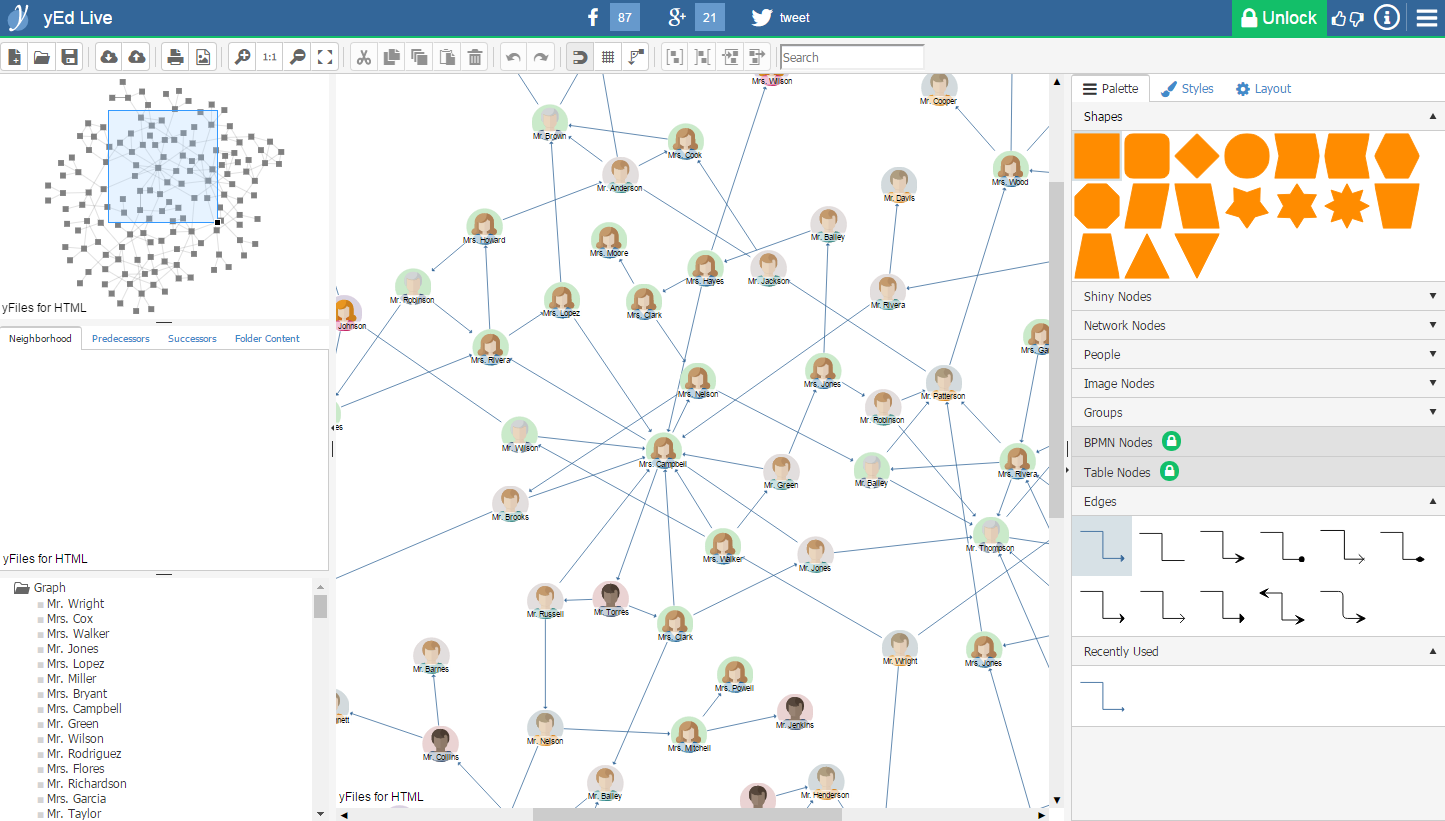
\includegraphics[width=\textwidth]{yed-live.png}
\caption{Zrzut ekranu z aplikacji yEd Live}
\end{figure}


\subsection*{Linkurious}
\bigskip
\noindent\begin{tabularx}{\textwidth}{r|X|}
\cline{2-2}
  Adres URL & http://linkurio.us \\ 
\cline{2-2} 
 Autor & Linkurious\\ 
\cline{2-2}
 Licencja & Płatna\\ 
\cline{2-2}
\end{tabularx}
\bigskip

Komercyjna aplikacja internetowa służąca do wizualizacji i badania grafowych baz danych\footnote{Wspierane bazy danych: \textit{Neo4j}, \textit{DataStax Enterprise Graph}, \textit{Titan}, \textit{AllegroGraph} oraz ich języki zapytań: \textit{Cypher}, \textit{Gremlin} i \textit{SPARQL}.}. Jej współzałożycielem jest Dr Sébastien Heymann -- współtwórca aplikacji desktopowej Gephi służącej również do wizualizacji i analizowania grafów. 

Aplikacja wspiera duże zbiory danych -- grafy z miliardami wierzchołków i krawędzi \cite{linkurious}. Pozwala na współpracę wielu użytkowników, m.in. przez możliwość udostępniania grafów czy publikowanie wizualizacji w czasie rzeczywistym. 

Posiada kilka opcji układów grafów (kierowanych siłą i hierarchicznych). Dostarcza również możliwość widoku geoprzestrzennego. 

W \textit{Linkurious} istnieje możliwość dostosowania wyglądu elementów, np. wielkość wierzchołków, grubość krawędzi, zmiana ikon w wierzchołkach, tak aby wizualizacje były bogate w informacje. Użytkownik może również tworzyć filtry, by wyświetlić tylko istotne dane oraz tworzyć powiadomienia o podejrzanych połączeniach. 

\begin{figure}[H]
\centering
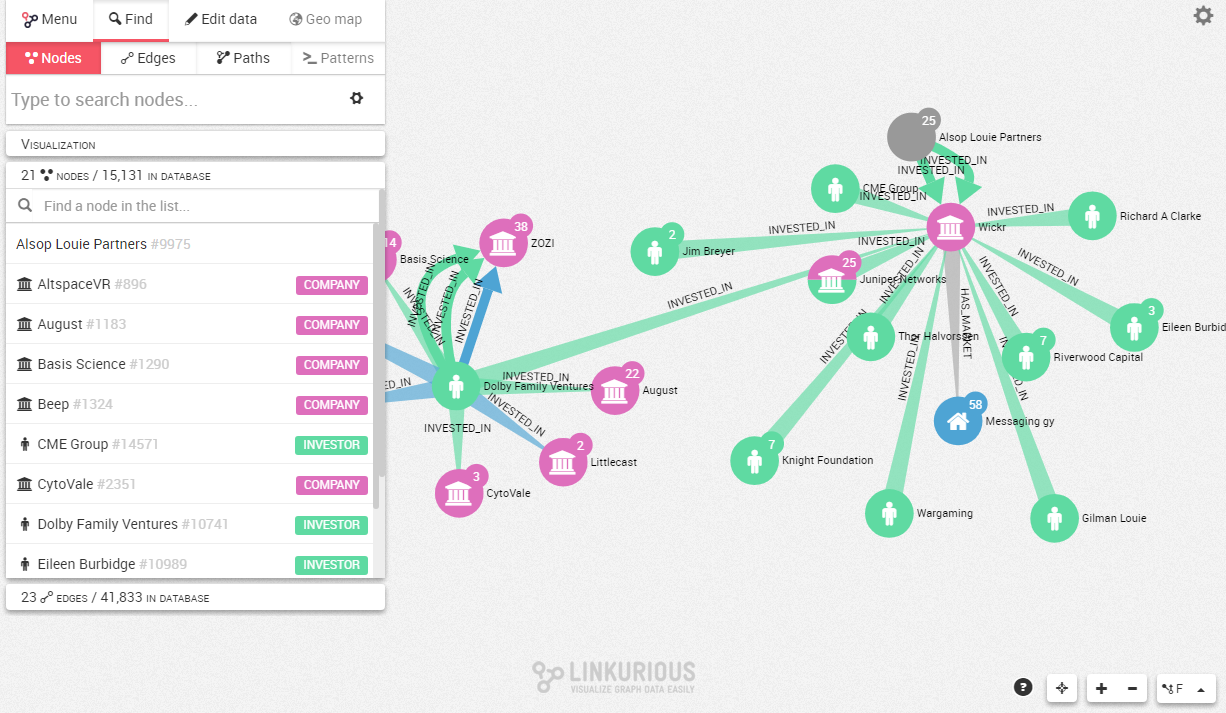
\includegraphics[width=\textwidth]{linkurious.png}
\caption{Zrzut ekranu z aplikacji Linkurious}
\end{figure}

\begin{table}[H]
\centering
\begin{threeparttable}
\caption{Porównanie darmowych aplikacji oraz aplikacji \emph{Graphy} -- tworzonej w ramach tej pracy}
\label{tab:app-comparison}
\begin{tabu}{ r|c|c|c|c|c|c| } 
\multicolumn{1}{r}{}
 &  \multicolumn{1}{c}{\rotatebox{80}{Graph Creator}}
 & \multicolumn{1}{c}{\rotatebox{80}{Graph Online}} 
 & \multicolumn{1}{c}{\rotatebox{80}{GraphJS}} 
 & \multicolumn{1}{c}{\rotatebox{80}{Graphrel}} 
 & \multicolumn{1}{c}{\rotatebox{80}{yEd Live}}
 & \multicolumn{1}{c}{\rotatebox{80}{Graphy}} \\
\cline{2-6}\tabucline[2pt]{7-7}
graf nieskierowany & \checkmark & \checkmark  & \checkmark  & -- & \checkmark & \Thickvrule{\checkmark} \\
\cline{2-7}
graf skierowany  & \checkmark & \checkmark  & --  & \checkmark & \checkmark & \Thickvrule{\checkmark} \\
\cline{2-7}
multigraf  & \checkmark & --  & \checkmark  & -- & \checkmark & \Thickvrule{\checkmark} \\
\cline{2-7}
etykiety na krawędziach  & \checkmark & \checkmark  & \checkmark  & -- & \checkmark & \Thickvrule{\checkmark}\\
\cline{2-7}
etykiety w wierzchołkach & \checkmark & \checkmark  & \checkmark  & -- & \checkmark & \Thickvrule{\checkmark} \\
\cline{2-7}
kolorowanie wierzchołków & \checkmark & --  & --  & -- & \checkmark & \Thickvrule{\checkmark} \\
\cline{2-7}
łuki jako krawędzie & \checkmark & --  & --  & -- & \checkmark & \Thickvrule{\checkmark} \\
\cline{2-7}
zaznaczanie kilku wierzchołków & \checkmark & --  & \checkmark  & -- & \checkmark & \Thickvrule{\checkmark} \\
\cline{2-7}
grupowanie wierzchołków & -- & --  & --  & -- & \checkmark & \Thickvrule{\checkmark} \\
\cline{2-7}
przesuwanie widoku & -- & \checkmark  & --  & -- & \checkmark & \Thickvrule{\checkmark} \\
\cline{2-7}
przybliżanie/oddalanie & -- & \checkmark  & --  & -- & \checkmark & \Thickvrule{\checkmark} \\
\cline{2-7}
zapisywanie/wczytywanie & -- & \checkmark\tnote{1}  & \checkmark\tnote{2}  & \checkmark\tnote{3} & \checkmark\tnote{4} & \Thickvrule{\checkmark} \\
\cline{2-7}
algorytmy & -- & \checkmark  & -- & -- & -- & \Thickvrule{\checkmark} \\
\cline{2-6}\tabucline[2pt]{7-7}
\end{tabu}
\begin{tablenotes}
{\footnotesize\bigskip
\item[1] jako macierz sąsiedztwa lub jako obrazek
\item[2] własny format \texttt{JSON} lub jako \LaTeX
\item[3] własny format (listy sąsiedztwa)
\item[4] \texttt{GraphML} lub jako obrazek (w wersji darmowej jest ograniczenie na
 wielkość zapisywanego grafu)
}
\end{tablenotes}
\end{threeparttable}
\end{table}

\section{Aplikacje desktopowe}

Istnieje również szereg aplikacji desktopowych służących do wizualizacji, analizy i edycji grafów. Są one bardziej rozbudowane i zakres ich funkcjonalności jest znacznie szerszy od aplikacji internetowych. Do najbardziej znanych należą \cite{mathex-desktop}:

\begin{itemize}
\setlength\itemsep{0em}
\item \href{https://gephi.org/}{Gephi}
\item \href{http://www.graphtheorysoftware.com/}{GraphTea}
\item \href{http://www.cytoscape.org/}{Cytoscape}
\item \href{https://www.yworks.com}{yEd Graph Editor}
\end{itemize}

\begin{figure}[H]
\centering
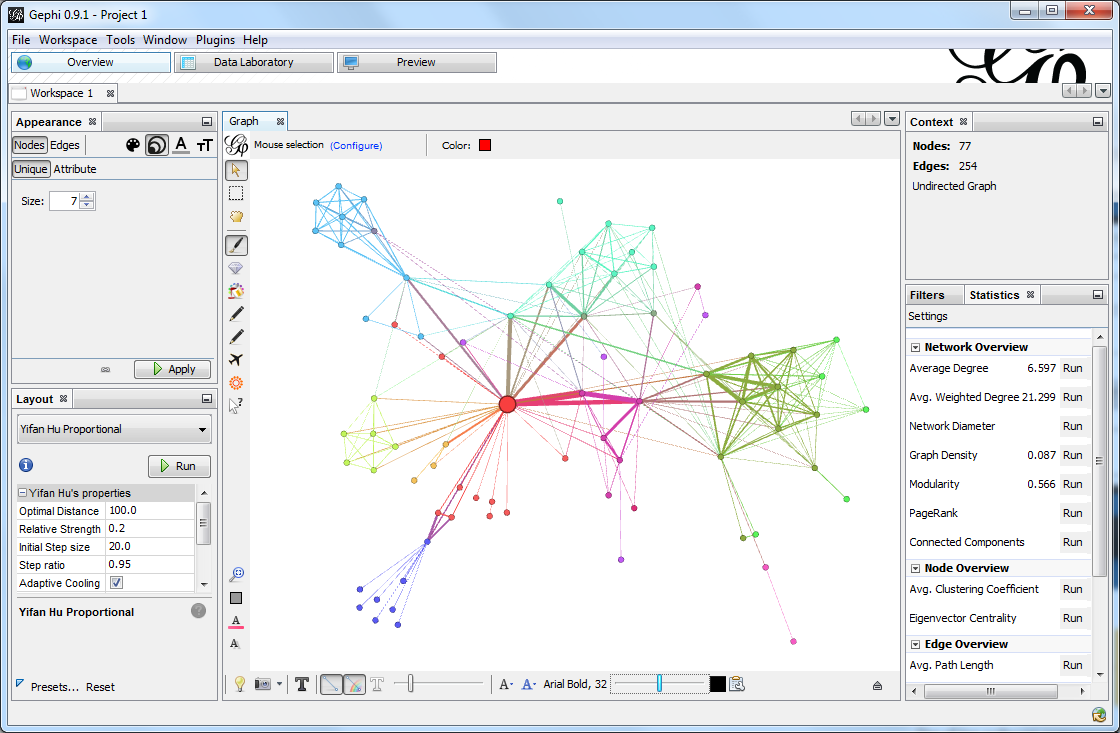
\includegraphics[width=\textwidth]{gephi.png}
\caption{Zrzut ekranu z aplikacji Gephi}
\end{figure}

\chapter{Przegląd dziedziny}
\section{Formaty zapisu grafów} \label{sec:graph-formats}
Istnieje wiele formatów służących do opisu grafów. Do najpopularniejszych należą \cite{bernard,gephi}

\begin{itemize}
\setlength\itemsep{0em}
\item \texttt{GraphML} -- \textit{Graph Markup Language}
\item \texttt{GEXF} -- \textit{Graph Exchange XML Format}
\item \texttt{JGF} -- \textit{JSON Graph Format}
\item \texttt{DOT} -- format programu Graphviz
\item \texttt{GML} -- \textit{Graph Modeling Language }
\item \texttt{DGML} -- \textit{Directed Graph Markup Language}
\item \texttt{XGMML} -- \textit{eXtensible Graph Markup and Modeling Language}
\end{itemize}

\subsubsection{Graph Markup Language (GraphML)}
\begin{listing}[H]
    \caption{Przykład grafu w formacie GraphML}
    \inputminted{xml}{example.graphml}
    \label{lst:graphml-example}
\end{listing}

\subsubsection{Graph Exchange XML Format (GEXF)}
\begin{listing}[H]
    \caption{Przykład grafu w formacie GEXF}
    \inputminted{xml}{example.gexf}
    \label{lst:gexf-example}
\end{listing}

\subsubsection{JSON Graph Format (JGF)} 
\begin{listing}[H]
    \caption{Przykład grafu w formacie JGF}
    \inputminted{json}{example.json}
    \label{lst:jgf-example}
\end{listing}

\subsubsection{DOT Graphviz} 
\begin{listing}[H]
    \caption{Przykład grafu w formacie DOT}
    \inputminted{text}{example.gv}
    \label{lst:dot-example}
\end{listing}

\section{Biblioteki do wizualizacji grafów w JavaScript}

\subsection{Cytoscape.js}

Biblioteka z otwartym źródłem (ang. \textit{open-source}) do analizy i wizualizacji grafów. Udostępniona na zasadach licencji MIT. Została napisana w czystym JavaScript i nie posiada zależności do żadnych innych bibliotek. Cytoscape.js jest następcą porzuconego projektu Cytoscape Web korzystającego z technologii Adobe Flash \cite[309]{franz}. 

Prawa własności intelektualnej posiada do niej Cytoscape Consortium -- organizacja non-profit, która promuje rozwój i dystrybucję oprogramowania związanego z sieciami biologicznymi. Cytoscape.js została stworzona na University of Toronto. Jej głównym kontrybutorem jest Max Franz. Biblioteka została sfinansowana przez granty NRNB (\textit{National Resource for Network Biology}) i NIH (\textit{National Institutes of Health}). Kilka innych uniwersytetów oraz firm również pomagało w rozwoju biblioteki \cite{cytoscape}. 

Cytoscape.js jest kompatybilny z kilkoma przydatnymi bibliotekami oraz środowiskami JavaScript, takimi jak: Node.js, Browserify, webpack, RequireJS czy Bower, co pozwala na integrację z szeroką gamą systemów opartych na JS. 

Architektura Cytoscape.js pozwala na uruchomienie zarówno bez graficznego interfejsu użytkownika oraz jako komponent graficzny, którego implementacja bazuje na elemencie HTML5 Canvas. Umożliwia to korzystanie z biblioteki zarówno po stronie klienta (np. przeglądarka internetowa), jak i po stronie serwera (np. Node.js).


\subsection{sigma.js}
\subsection{VivaGraph.js}
\subsection{Linkurious.js}

\begin{table}[H]
\begin{tabularx}{\textwidth}{|r|c|c|c}
\hline 
 & Cytoscape.js & Sigma & VivaGraphJS \\ 
\hline 
Licencja & MIT & MIT & BSD 3 \\ 
\hline 
Rozmiar & 294 & 112,9 & 60,4 \\ 
\hline 
Renderowanie & & & \\
SVG & • & tak & • \\
HTML5 Canvas & • & tak & • \\
WebGL Canvas & • & tak & • \\ 
\hline 
Obsługiwane formaty & • & • & • \\ 
\hline
Rozszerzalność & • & • & • \\ 
\hline 
• & • & • & • \\ 
\hline 
\end{tabularx} 
\end{table}



\chapter{Projekt aplikacji}\label{ch:project}

W tym rozdziale przedstawię wszystkie wymagania funkcjonalne, które powinna spełniać aplikacja, aby użytkownik miał możliwość stworzyć graf dowolnego typu, wyświetlić go w optymalny sposób (wraz z możliwością zmiany widoku) oraz zmienić graf w dowolny sposób, np. poprzez dodawanie nowych wierzchołków i krawędzi, czy edycję etykiet. 

Opiszę również wymagania niefunkcjonalne, aby praca z grafami była możliwie przystępna. Uwzględnię m.in.: wydajność, wspierane platformy, wygodną obsługę przez użytkownika oraz łatwą rozszerzalność dla programistów (co zostanie osiągnięte na przykład poprzez modułowowść kodu w JavaScript).

Na koniec rozdziału zaprezentuję prototyp graficznego interfejsu użytkownika uwzględniającego wszystkie wymagania funkcjonalne, który będzie obrazował jak powinna wyglądać aplikacja tworzona w ramach tej pracy. 

\section{Wymagania funkcjonalne}

\subsection{Tworzenie grafów}
Podstawowym i oczywistym wymaganiem jest, aby użytkownik mógł stworzyć nowy, pusty graf skierowany oraz nieskierowany. Ponadto użytkownik powinien mieć możliwość zaimportowania istniejącego grafu oraz wygenerowania znanego grafu, np. cyklu lub grafu pełnego o zadanej ilości wierzchołków. 

\subsubsection{Importowanie grafów} \label{subsubsec:import}
Użytkownik powinien móc wczytać graf z komputera lub z chmury (np. Google Drive lub Dropbox) w trzech znanych formatach: 

\begin{itemize}
\setlength\itemsep{0em}
\item \texttt{GraphML},
\item \texttt{GEXF},
\item \texttt{JGF}.
\end{itemize}

Opisy formatów znajdują się w sekcji \ref{sec:graph-formats}.

\subsubsection{Generowanie grafów}

Użytkownik powinien mieć możliwość wygenerowania znanych grafów, dla zadanych parametrów wejściowych:

\begin{itemize}
\setlength\itemsep{0em}
\item grafu pustego,
\item grafu liniowego,
\item grafu cyklicznego,
\item koła,
\item grafu pełnego (lub turnieju dla grafów skierowanych),
\item grafu pełnego dwudzielnego,
\item grafu Petersena,
\item drzewa (o zadanej wysokości i ilości dzieci)
\end{itemize}

Definicje i przykłady powyższych grafów znajdują się w sekcji \ref{sec:common-graphs}.

Ponadto przydatnym dodatkiem w aplikacji będzie możliwość wygenerowania grafu losowego -- o danej ilości wierzchołków oraz parametrem prawdopodobieństwa określającym, czy pomiędzy dwoma wierzchołkami istnieje krawędź.  

\subsection{Wizualizacja}

Użytkownik powinien móc przesuwać widok, przybliżać i oddalać graf oraz rozmieszczać wierzchołki grafu w dowolny sposób. W aplikacji powinna istnieć możliwość zmiany układu grafu: układ oparty na oddziaływaniach (ang. \textit{force-based layout}), układ siatki, układ okręgu, układ koncentryczny, układ hierarchiczny. 

Użytkownik powinien być w stanie zmienić kategorię wierzchołka oraz typ krawędzi. Inne typy i kategorie powinny być oznaczone innym kolorem oraz powinna istnieć możliwość zmiany koloru. 

Aplikacja powinna również dostarczać opcję wyszukiwania i filtrowania danych (np. tylko dany typ wierzchołków, wierzchołki o stopniu większym niż zadany parametr). Przydatną funkcjonalnością będzie wyświetlanie sąsiadów danego wierzchołka po najechaniu na niego kursorem myszy.

\subsection{Edycja}

W aplikacji powinien istnieć osobny tryb edycji. Gdy użytkownik jest w tym trybie, powinien móc dodawać oraz usuwać wierzchołki i krawędzie. Powinien być w stanie także dodawać oraz modyfikować etykiety wierzchołków i krawędzi.

Użytkownik powinien mieć możliwość zaznaczania wielu wierzchołków i krawędzi na raz. Użyteczną funkcjonalnością będzie również grupowanie (lub rozgrupowanie) zaznaczonych wierzchołków. 

Aplikacja powinna wyświetlać ostatnio wykonaną akcję oraz udostępniać możliwość jej cofnięcia.

\subsection{Przetwarzanie}

Aplikacja powinna dawać możliwość wykonania podstawowych algorytmów na danym grafie:

\begin{itemize}
\setlength\itemsep{0em}
\item wyszukiwanie najkrótszej ścieżki pomiędzy dwoma wybranymi wierzchołkami,
\item znajdowanie minimalnego drzewa rozpinającego,
\item obliczanie algorytmu PageRank,
\item znajdowanie (silnie) spójnych składowych oraz dwuspójnych składowych,
\item znajdowanie cyklu Eulera,
\item znajdowanie cyklu Hamiltona.
\end{itemize}

\subsection{Eksportowanie}
Użytkownik powinien mieć możliwość wyeksportowania do formatów, które zostały przedstawione w podsekcji \ref{subsubsec:import}. 

Ponadto przydatną funkcjonalnością będzie możliwość wyeksportowania obecnego widoku do pliku graficznego, np. \texttt{PNG} lub \texttt{JPG}. 

\subsection{Udostępnianie grafu}
W aplikacji powinna istnieć możliwość udostępniania grafu innym użytkownikom. Po wybraniu tej opcji, powinien zostać wygenerowany unikalny odnośnik do grafu. Po przejściu na ten adres (w podstawowej wersji) inni użytkownicy mogą wyświetlić i edytować graf.


\section{Wymagania niefunkcjonalne}

\subsection{Wydajność}

Aplikacja powinna być w stanie efektywnie wyświetlać oraz modyfikować grafy. Małe grafy (mające do około 50 wierzchołków) powinny być wyświetlane od razu, podobnie modyfikacja takich grafów powinna być odzwierciedlana natychmiast. Podczas wyświetlania oraz edycji grafów średnich (mających od 50 do 1000 wierzchołków) dozwolone jest niewielkie opóźnienie, mieszące się w graniach od 300-1500 ms. 

Aplikacja powinna obsługiwać również duże grafy (mające np. 1 milion wierzchołków). W przypadku takich grafów dozwolone są opóźnienia jednakże ich postęp powinien być przedstawiany użytkownikowi, interfejs nie powinien być blokowany oraz użytkownik powinien mieć możliwość anulowania zbyt długo trwających operacji. Przydatną funkcjonalnością będzie również powiadamianie użytkownika o akcji, która może zająć dłuższy czas (np. powyżej 5 sekund).

System powinien być w stanie obsługiwać wielu użytkowników -- wzrost liczby użytkowników nie powinien mieć większego wpływu na responsywność oraz szybkość odpowiedzi. Wymaganie to powinno być spełnione w łatwy sposób, ponieważ większość operacji (choć nie wszystkie) będzie wykonywana po stronie klienta (w przeglądarce internetowej). Dla tych operacji, które nie będą wykonywane na komputerze użytkownika, rozsądnym wymaganiem jest, aby część serwerowa była łatwo skalowalna.

\subsection{Wspierane platformy}

Część kliencka aplikacji powinna działać na wszystkich popularnych systemach operacyjnych (Windows, Linux, Mac OS) oraz przeglądarkach (Google Chrome, Mozilla Firefox, Internet Explorer, Safari, Opera). Jeśli chodzi o część serwerową, to również powinna istnieć możliwość uruchomienia jej pod dowolnym system operacyjnym.

Ze względu na wzrost znaczenia urządzeń mobilnych powinna być możliwość łatwego korzystania z aplikacji na ów urządzeniach (zwłaszcza na tabletach, które posiadają na tyle duży ekran, aby móc wygodnie wyświetlić graf i edytować go). By było to możliwe aplikacja musi: po pierwsze, automatycznie dostosowywać się do rozmiaru okna (ang. \textit{Responsive Web Design}); po drugie, wspierać gesty obsługiwane przez urządzenia przenośne, np. przeciągnięcie, wykorzystanie dwóch palców, przytrzymanie elementu na ekranie. 

\subsection{Użyteczność}

Aplikacja powinna spełniać kryteria użyteczności (ang. \textit{usability}), aby praca z nią była jak najbardziej intuicyjna, prosta i przyjemna. Jakob Nielsen podaje 5 elementów, które wchodzą w skład użyteczności \cite{nielsen}:

\begin{itemize}
\setlength\itemsep{1em}
\item \textbf{Nauczalność} (ang. \textit{learnability}) -- jak łatwa jest dla użytkowników realizacja podstawowych zadań, gdy po raz pierwszy korzystają z aplikacji? 

Dla nowych użytkowników powinny wyświetlać się podpowiedzi, które pozwolą im jak najszybciej nauczyć się obsługi programu. Dla użytkowników, którzy uruchomią aplikację po raz pierwszy powinien otworzyć się krótki (opcjonalny) przewodnik, który oprowadzi ich po aplikacji i zapozna z wszystkimi dostępnymi funkcjonalnościami.

\item \textbf{Efektywność} (ang. \textit{efficiency}) -- gdy użytkownicy znają program, jak szybko mogą wykonywać zadania?

Aplikacja powinna oferować skróty klawiszowe, które przyspieszą pracę zaawansowanych użytkowników. W menu powinna być opcja wyświetlenia wszystkich skrótów klawiszowych oraz powinny być one podpowiadane użytkownikowi przy starcie lub podczas korzystania z programu.

\item \textbf{Zapamiętywalność} (ang. \textit{memorability}) -- jak łatwo użytkownicy mogą przywrócić biegłość korzystania z aplikacji, gdy powracają do niej po dłuższej przerwie?

Użytkownik powinien mieć możliwość ponownego włączenia podpowiedzi, przewodnika oraz wyświetlenia listy wszystkich dostępnych skrótów klawiszowych. 

\item \textbf{Błędy} (ang. \textit{errors}) -- jak wiele błędów popełniają użytkownicy, jak poważne są te błędy, jak łatwo mogą je poprawić?

Możliwość popełnienia błędu powinna być zminimalizowana do zera, np. poprzez specjalny tryb edycji użytkownik nie jest w stanie przypadkowo dodać nowy wierzchołek. Ponadto po każdej akcji modyfikującej powinno wyświetlić się powiadomienie (ang. \textit{toast}, \textit{snack-bar}) mówiące o tym, w jaki sposób graf się zmienił oraz przycisk z opcją cofnięcia ostatnio wykonanej operacji. Powinna istnieć również opcja cofania ostatnich akcji i ponawiania ich korzystając ze znanych skrótów klawiszowych \texttt{Ctrl+Z} oraz \texttt{Ctrl+Y}. 

\item \textbf{Satysfakcja} (ang. \textit{satisfaction}) -- jak przyjemne jest korzystanie z programu?

Wszystkie przedstawione powyżej wymagania funkcjonalne i niefunkcjonalne powinny przyczynić się do tego, że użytkownik będzie mógł w łatwy i przyjemny sposób tworzyć, wyświetlać i edytować swoje grafy.

\end{itemize}

\subsection{Rozszerzalność}

Aplikacja zostanie udostępniona na zasadach otwartego oprogramowania (ang. \textit{open source}). Dlatego tez powinna w łatwy sposób dać się rozszerzać przez innych programistów, dając możliwość np. dodawania nowych algorytmów, sposobów importowania oraz eksportowania grafów, czy obsługi nowych formatów. 

Rozszerzalność będzie zapewniona przede wszystkim przez: 
\begin{itemize}
\setlength\itemsep{0em}
\item strukturę i modułowość kodu, 
\item dokumentację interfejsów aplikacji i opis architektury systemu, 
\item przykłady w jaki sposób zrealizować znane problemy, 
\item wysokie pokrycie testami jednostkowymi i integracyjnymi, które zagwarantują, że modyfikacja kodu nie zepsuje istniejących już funkcjonalności. 
\end{itemize}

\pagebreak

\section{Prototyp interfejsu użytkownika}

\subsection*{Tryb widoku grafu}

Graf powinien być wyświetlony w całym oknie przeglądarki. U góry po lewej powinno znajdować się rozsuwane menu, a obok niego przyciski: \textit{Edycja}, \textit{Wyszukaj} i \textit{Algorytmy}. Z kolei po stronie prawej powinien znajdować się pływający przycisk (ang. \textit{floating button}) wyświetlający informację o zalogowanym użytkowniku i dający możliwość wyświetlić menu użytkownika. 

Na dole po prawej stronie powinno znajdować się menu z opcjami zmieniającymi widok grafu (przybliżanie i oddalanie, zmiana układu, włączenie i wyłączenie oddziaływania pomiędzy wierzchołkami).

Gdy nie ma otwartego żadnego grafu, to w tle powinny pojawiać się podpowiedzi ze skrótami klawiszowymi, które co kilka sekund będą się zmieniać. 

\vspace*{\fill}
\begin{figure}[H]
\centering
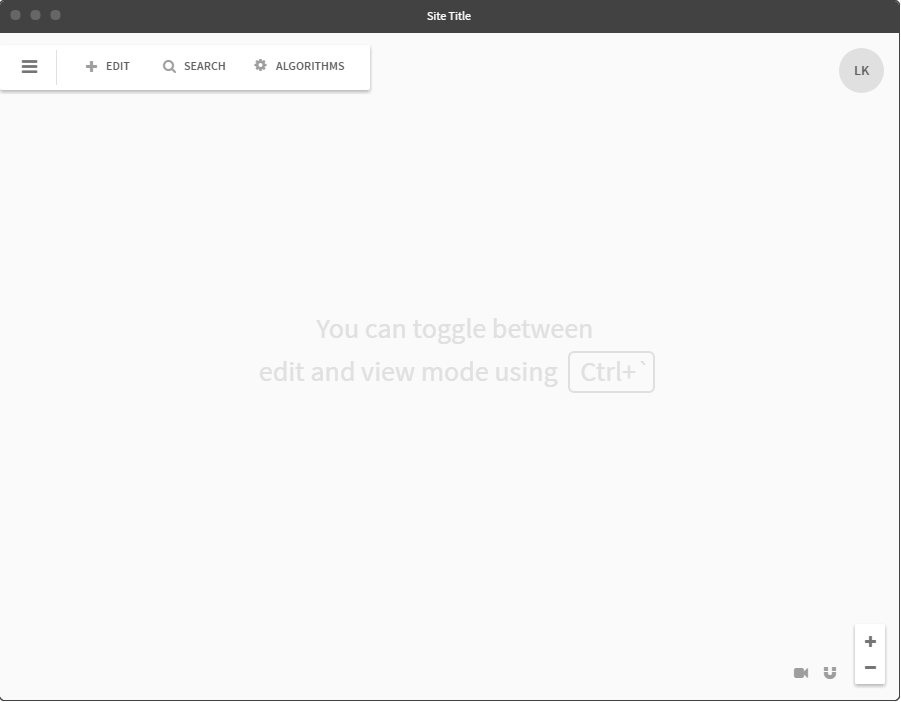
\includegraphics[width=\textwidth]{mock-view.png}
\caption{Tryb widoku grafu}
\end{figure}
\vspace*{\fill}

\pagebreak

\subsection*{Tryb edycji grafu}

Użytkownik powinien być poinformowany, że jest w trybie edycji poprzez oznaczenie przycisku oraz obramowania okna wyróżniającym się kolorem.

\vspace*{\fill}
\begin{figure}[H]
\centering
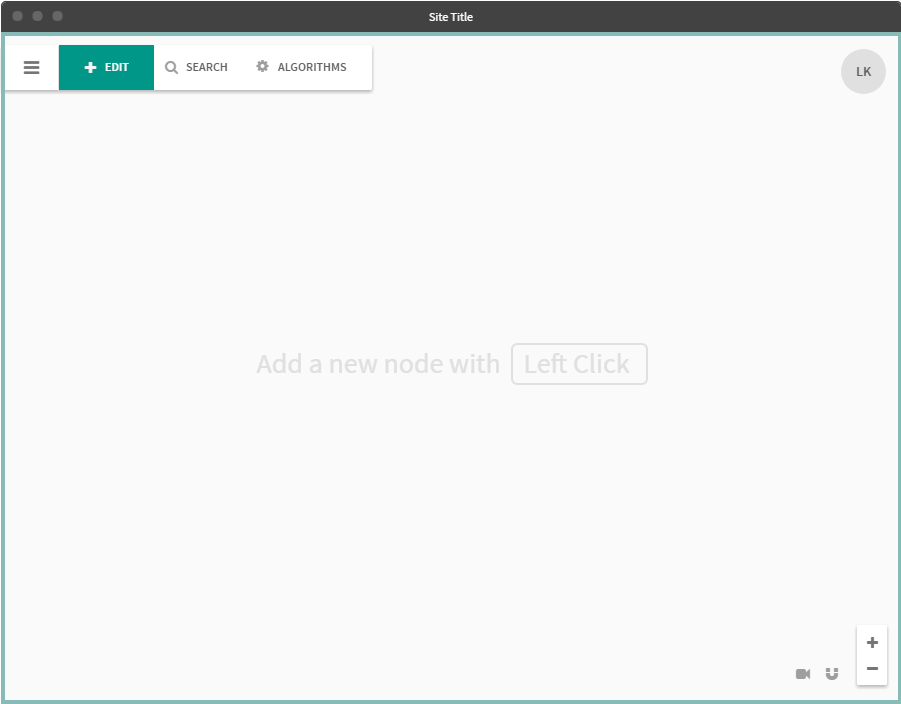
\includegraphics[width=\textwidth]{mock-edit.png}
\caption{Tryb edycji grafu}
\end{figure}
\vspace*{\fill}

\pagebreak

\subsection*{Widok menu}

Menu powinno wysuwać się z boku, a pod nim powinna pojawić się warstwa z półprzezroczystym tłem. Powinno oferować podstawowe opcje tworzenia nowego grafu, otwierania zapisanego grafu, udostępniania czy eksportowania. W menu powinny znaleźć się też takie opcje jak: wyświetlenie listy skrótów, zmiana języka, kontakt czy możliwość zgłoszenia błędu w aplikacji oraz informacja o prawach autorskich.

\vspace*{\fill}
\begin{figure}[H]
\centering
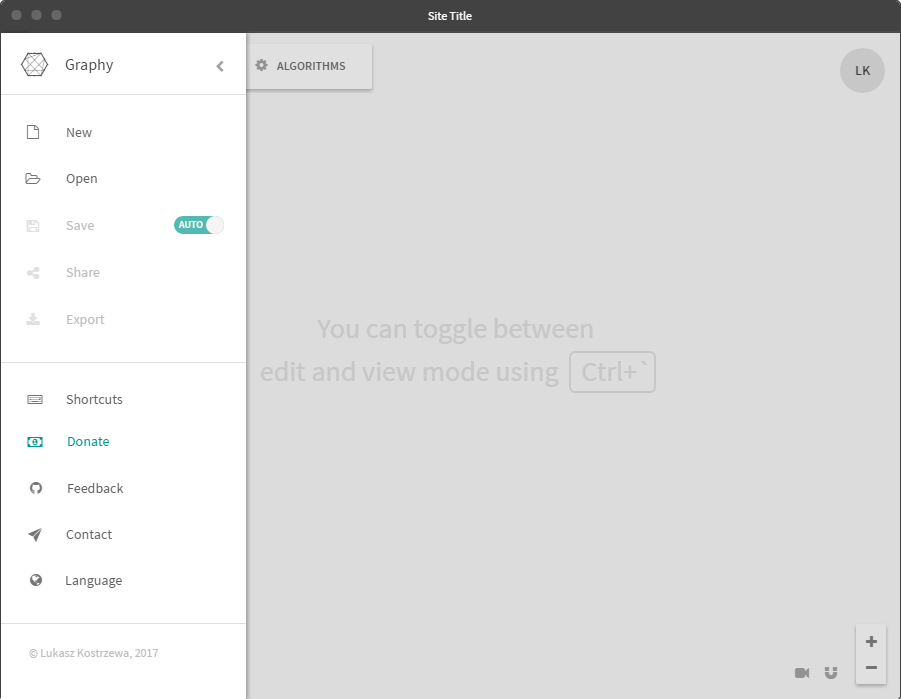
\includegraphics[width=\textwidth]{mock-menu.png}
\caption{Widok menu}
\end{figure}
\vspace*{\fill}

\pagebreak

\subsection*{Menu kontekstowe i informacja o ostatniej akcji}

Po kliknięciu prawego klawisza myszy powinno pojawić się niestandardowe menu kontekstowe zawierające dodatkowe opcje pozwalające na edycję, usuwanie, zaznaczanie, grupowanie, wycinanie, kopiowanie, wklejanie wierzchołków i krawędzi oraz na cofanie i ponawianie ostatniej akcji.

Po wykonaniu akcji modyfikującej graf na dole strony powinno wyświetlić się powiadomienie o wykonaniu tej akcji z przyciskiem umożliwiającym jej cofnięcie. 

\vspace*{\fill}
\begin{figure}[H]
\centering
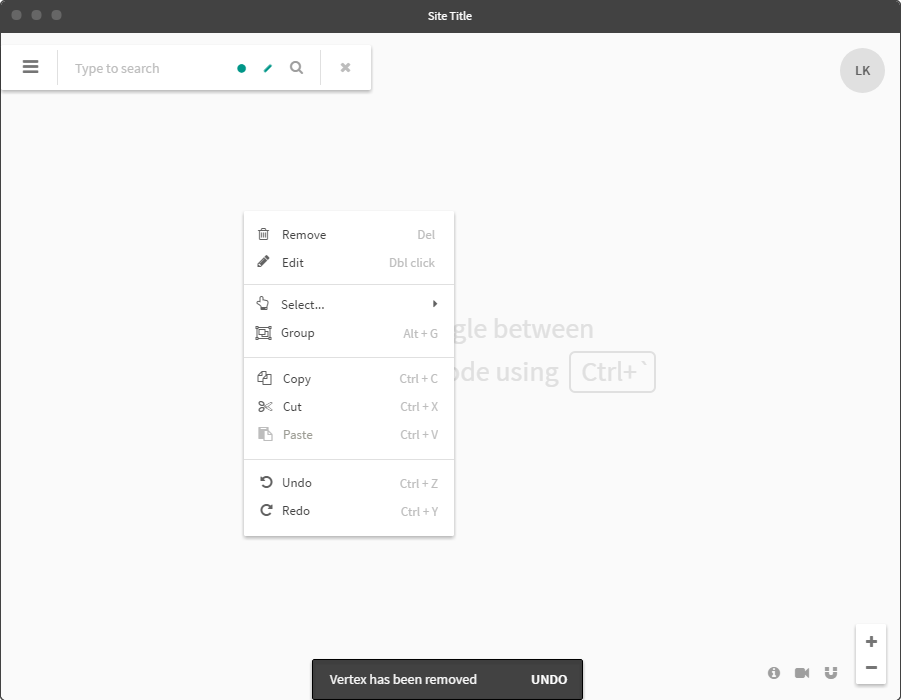
\includegraphics[width=\textwidth]{mock-context-menu.png}
\caption{Menu kontekstowe i informacja o ostatniej akcji}
\end{figure}
\vspace*{\fill}
\chapter{Implementacja}

Rozdział ten zawiera wszystkie informacje dotyczące aplikacji noszącej nazwę Graphy, która została napisana w ramach tej pracy. 

Przedstawię w nim użyte narzędzia i biblioteki oraz architekturę systemu. Opiszę również działanie aplikacji: które funkcjonalności udało mi się zaimplementować, a które wymagają dalszej pracy. 

Znajdzie się tutaj również sekcja o testach aplikacji (jednostkowych, \textit{end-to-end} oraz manualnych). Następnie pojawią się bardziej techniczne informacje dla programistów, opisujące w jaki sposób zrealizować typowe zadanie takie jak np. dodanie nowego parsera czy algorytmu. Na samym końcu przedstawię pomysły, w jaki sposób można dalej rozwijać aplikację.

\section{Podstawowe informacje}

Aplikacja została napisana w języku TypeScript -- wolnym i otwartym języku programowania stworzonym przez firmę Microsoft, który jest nadzbiorem języka JavaScript i który transpiluje się do JavaScriptu. Umożliwia on statyczną kontrolę typów oraz programowanie zorientowane obiektowo oparte na klasach.

Projekt korzysta z systemu kontroli wersji Git i jego repozytorium kodu znajduje się w serwisie GitHub. Wersja demonstracyjna aplikacji jest udostępniona na serwerach GitHub Pages. Adresy repozytorium i wersji demonstracyjnej znajdują się w poniższej tabeli.

\bigskip\bigskip
\noindent\begin{tabularx}{\textwidth}{r|X|}
\cline{2-2}
  Repozytorium kodu & \hyperref[https://github.com/lukaszkostrzewa/graphy]{https://github.com/lukaszkostrzewa/graphy} \\ 
\cline{2-2} 
 Wersja demonstracyjna & \hyperref[https://lukaszkostrzewa.github.io]{https://lukaszkostrzewa.github.io} \\ 
\cline{2-2}
\end{tabularx} 
\bigskip\bigskip

Jest to aplikacja \textit{front-endowa}. Oznacza to, że w chwili obecnej nie komunikuje się ona z serwerem ani zewnętrznymi serwisami (np. w celu zapisania czy zaimportowania grafu). Wszystkie operacje są wykonywane po stronie klienta, tzn. po stronie przeglądarki internetowej. Przy dalszym rozwoju aplikacji konieczne może okazać się napisanie drugiej, odseparowanej aplikacji pełniącej rolę \textit{back-endu}, która będzie wystawiać serwisy umożliwiające komunikację z bazą danych czy z innymi użytkownikami (np. udostępnianie grafu w czasie rzeczywistym).

Aplikacja została udostępniona na licencji MIT. Poniższa tabela przedstawia podstawowe statystyki dotyczące projektu.

\bigskip
\begin{table}[H]
\begin{threeparttable}
\centering
\noindent\begin{tabularx}{\textwidth}{r|X|}
\cline{2-2}
  Liczba linii kodu\tnote{1} & 8137 \\ 
\cline{2-2}
  Liczba plików\tnote{1} & 151 \\ 
\cline{2-2}
 Rozmiar kodu\tnote{1} & 270 KB \\ 
\cline{2-2}
 Ilość zatwierdzonych zmian w Git\tnote{2} & 112 \\ 
\cline{2-2}
 Pokrycie testami jednostkowymi\tnote{3} & 74.57\% \\ 
\cline{2-2}
\end{tabularx} 
\begin{tablenotes}
{\footnotesize\medskip
\item[1] nie licząc kodu zewnętrznych bibliotek
\item[2] ang. \textit{commits}
\item[3] procent pokrytych linii kodu
}
\end{tablenotes}
\end{threeparttable}
\end{table}
\bigskip


\section{Biblioteki i narzędzia}

W aplikacji jako biblioteka do wizualizacji grafów została użyta biblioteka Cytoscape.js. Posiada ona bardzo przyjazne API, obszerną dokumentację zawierającą gotowe przykłady oraz szereg dodatków, które rozszerzają podstawowe funkcjonalności. Ogromnym plusem biblioteki jest to, że jest aktywnie rozwijana, posiada dużą społeczność i wsparcie -- jej główny kontrybutor Max Franz odpowiada na każdą wiadomość w serwisach Stack Overflow oraz GitHub. Kolejnymi zaletami są architektura biblioteki oraz wsparcie dla urządzeń mobilnych.

Aplikacja została napisana przy użyciu biblioteki Angular, która została stworzona i jest rozwijana przez firmę Google. Projekt został wygenerowany przez narzędzie Angular CLI (ang. \textit{command line interface}). Narzędzie to umożliwia szybki start z biblioteką Angular -- pozwala na wygenerowanie już skonfigurowanego projektu, dostarcza komendy do generowania nowych komponentów, serwisów czy dyrektyw, do uruchamiania testów jednostkowych oraz testów \textit{end-to-end} oraz zawiera w sobie serwer programistyczny, który oferuje możliwość automatycznego przeładowywania aplikacji po wykryciu zmiany w kodzie źródłowym. 

Angular w wersji 2 (i nowszej) korzysta z języka TypeScript. Dzięki niemu i dzięki statycznej kontroli typów, którą język ten oferuje, możemy wcześniej uniknąć błędów programistycznych, już w momencie pisania kodu, a nie w momencie uruchomienia. Ponadto język ten oferuje szereg elementów z nadchodzących edycji ECMAScript\footnote{ECMAScript -- specyfikacja skryptowego języka stworzona i rozwijana przez organizację Ecma International, którą implementuje m.in. JavaScript.} takich jak moduły, klasy, interfejsy oraz wiele innych. Pozwala to na pisanie kodu modułowego, który jest łatwiejszy w utrzymaniu, testowaniu i rozwijaniu.

Ponadto w projekcie wykorzystywane są narzędzia do testowania domyślnie dostarczane w projekcie wygenerowanym przez Angular CLI: Karma i Protractor. Ich dokładniejszy opis znajduje się w sekcji \ref{sec:tests} Testy.

\section{Architektura}

Projekt składa się z 19 \emph{komponentów} (\texttt{@Component}). Każdy komponent mieści się w osobnym katalogu, w którym (zgodnie z konwencją zalecaną w Angularze) znajdują się: 
\begin{itemize}
\setlength\itemsep{0em}
\item plik \texttt{*.html} odpowiadający za widok, 
\item plik \texttt{*.scss} będący arkuszem styli Sass\footnote{Sass (ang. \textit{Syntactically Awesome Style Sheets}) -- jest to rozszerzenie języka CSS wzbogacającym go o takie funkcjonalności jak dziedziczenie, zagnieżdżanie styli, stosowanie zmiennych czy importowanie styli z innych plików.}, 
\item plik \texttt{*.ts} zawierający kod z klasą komponentu,
\item oraz plik \texttt{*.spec.ts} z testami jednostkowymi komponentu. 
\end{itemize}

Głównym komponentem jest \texttt{GraphComponent}, w którym jest inicjalizowany obiekt Cytoscape. Korzysta on z \emph{serwisów} (\texttt{@Injectable}), aby zaimportować graf, wyeksportować graf lub uruchomić na nim algorytm.

Oprócz tego w projekcie znajduje się szereg \emph{dyrektyw} (\texttt{@Directive}), które pełnią funkcję rozszerzeń (np. menu kontekstowe, dodatek odpowiadający za wyginanie krawędzi czy dodatek odpowiadający za rejestrację i obsługę skrótów klawiszowych).

Zarys architektury wraz z zaznaczonymi ważniejszymi komponentami, serwisami i dyrektywami został przedstawiony na rysunku \ref{fig:architecture}.

\begin{figure}[H]
\centerline{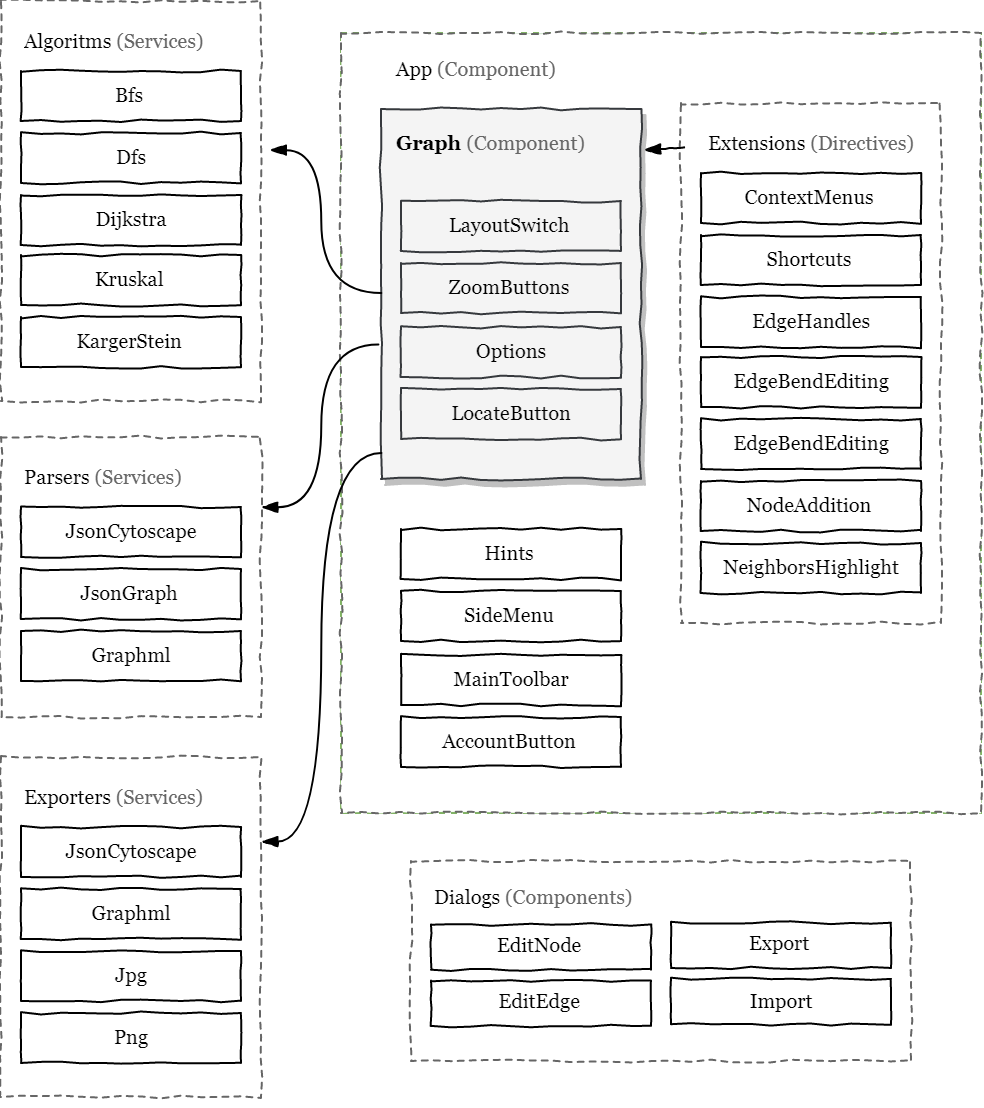
\includegraphics[width=1.1\textwidth]{architecture}}
\captionsetup{justification=centering,aboveskip=24pt}
\caption{Zarys architektury projektu \\ (niektóre komponenty zostały pominięte)}
\label{fig:architecture}
\end{figure}

\begin{figure}[H]
\centerline{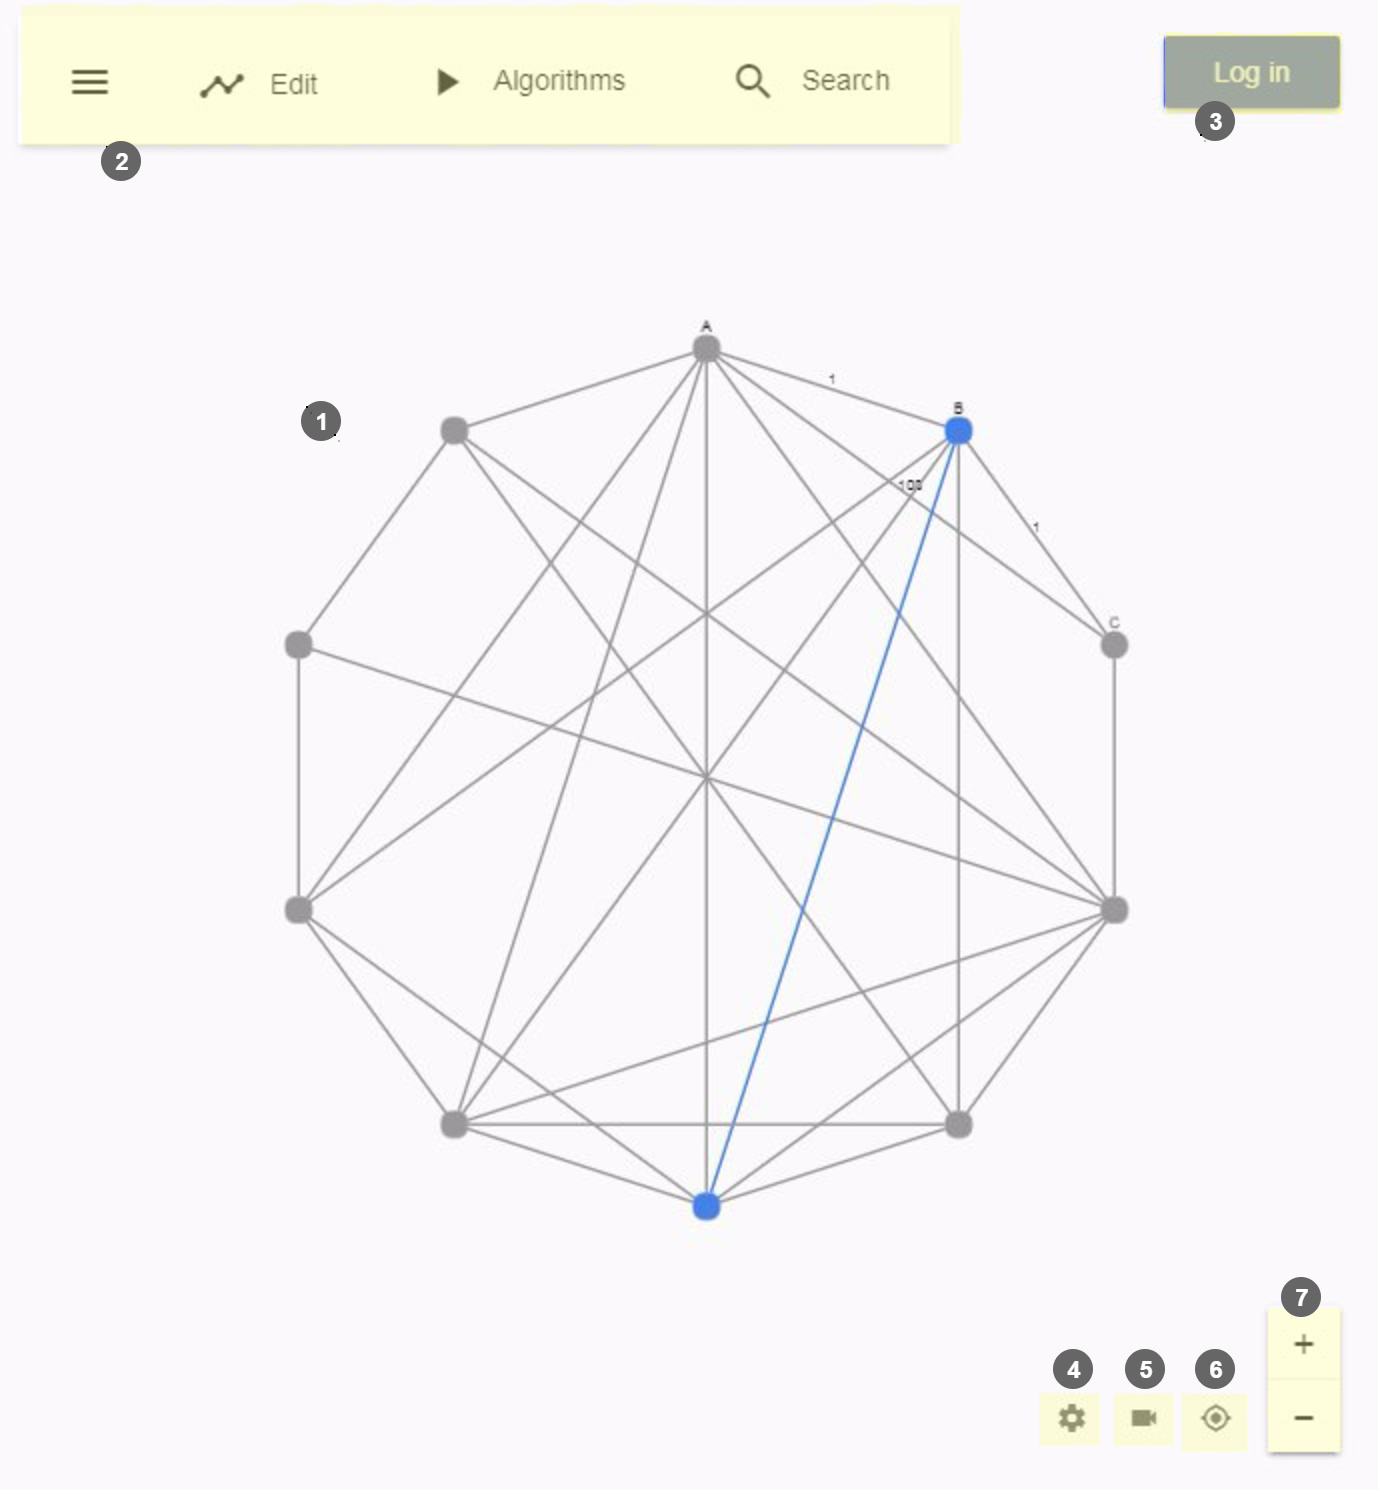
\includegraphics[width=1.0\textwidth]{graphy}}
\captionsetup{singlelinecheck=off}
\caption[Graphy]{
Aplikacja Graphy z zaznaczonymi głównymi komponentami:
\begin{enumerate}
\setlength{\itemsep}{0pt}
\setlength{\parskip}{2pt}
\item \texttt{GraphComponent}
\item \texttt{MainToolbarComponent}
\item \texttt{AccountButtonComponent}
\item \texttt{OptionsButtonComponent}
\item \texttt{LyoutSwitchComponent}
\item \texttt{LocateButtonComponent}
\item \texttt{ZoomButtonsComponent}
\end{enumerate}
}
\label{fig:graphy-app}
\end{figure}

\section{Zaimplementowane funkcjonalności}

W aplikacji udało się zaimplementować większość funkcjonalności, które zostały opisane w rozdziale \ref{ch:project} pt. ,,Projekt aplikacji''. Są to przede wszystkim:

\begin{itemize}
\setlength\itemsep{0em}
\item tworzenie grafów skierowanych oraz nieskierowanych,
\item importowanie grafu z formatów: GraphML, JSON Graph Format lub z~formatu JSON, z którego korzysta biblioteka Cytoscape.js,
\item eksportowanie do formatu GraphML, formatu JSON obsługiwanego przez Cytoscape.js oraz plików graficznych w formatach JPG i PNG,
\item obsługa podstawowych algorytmów wraz z animacją (BFS, DFS, algorytm Dijkstry, algorytm Kruskala, algorytm Kargera-Steina),
\item tryb edycji: dodawanie wierzchołków poprzez kliknięcie na obszar roboczy (lub z menu kontekstowego); dodawanie krawędzi poprzez przeciąganie (lub z menu kontekstowego),
\item grupowanie wierzchołków,
\item zmiana stylu wierzchołków oraz krawędzi (kolor, kształt, grubość krawędzi, styl linii, wielkość wierzchołków),
\item wyginanie krawędzi,
\item przystosowane menu kontekstowe,
\item obsługa skrótów klawiszowych,
\item wyświetlanie ostatniej akcji wraz z możliwością jej cofnięcia,
\item kopiowanie, wycinanie, wklejanie wierzchołków i krawędzi,
\item wsparcie dla urządzeń mobilnych i z ekranem dotykowym.
\end{itemize}

\section{Niezaimplementowane funkcjonalności i wizja dalszego rozwoju}

Jednakże ze względu na ograniczony czas i szeroki zakres pracy, nie wszystkie funkcjonalności udało się zaimplementować. Należą do nich głównie:

\begin{itemize}
\setlength\itemsep{0em}
\item logowanie użytkownika,
\item wczytywanie i zapisywanie grafów do bazy, na Dropboxie lub na Google Drive,
\item obsługa formatu GEXF,
\item generowanie grafów,
\item wyszukiwanie elementów w grafie,
\item ograniczona liczba algorytmów,
\item udostępnianie grafu,
\item wydajność i obsługa dużych grafów.
\end{itemize}

Logowanie użytkowników i zapis grafów do bazy będzie możliwe po zaimplementowaniu części serwerowej. Dzięki architekturze aplikacji, dodanie gotowego parsera nie powinno być wielkim wyzwaniem. To samo dotyczy dodawania nowych algorytmów. Warto wspomnieć, że jeszcze nie wszystkie algorytmy domyślnie zaimplementowane w bibliotece Cytoscape.js są obecnie wykorzystywane w aplikacji.

Jeśli chodzi o wydajność i obsługę dużych grafów, to nie zostało to sprawdzone. Niewykluczone, że przy dużych grafach aplikacja będzie działać powoli. Wówczas pomocne może okazać się zastosowanie wskazówek zawartych na stronie Cytoscape.js w sekcji dotyczącej wydajności (\cite{cytoscape} \textit{Performance}). Warto będzie również dopisać testy wydajności by móc ją na bieżąco kontrolować. 

Udostępnianie grafów innym użytkownikom w czasie rzeczywistym jest interesującym tematem. Aby to osiągnąć konieczne będzie również dopisanie części serwerowej. Przy obecnym stanie rzeczy, prawdopodobnie najlepszym rozwiązaniem będzie zastosowanie technologii WebSocket, która zapewnia dwukierunkową komunikację pomiędzy serwerem a przeglądarką internetową poprzez protokół TCP. 

Kolejnym interesującym i szerokim zagadnieniem jest integracja z grafowymi bazami danych, np. z bazą Neo4j poprzez protokół Bolt i język zapytań Cypher.

\bigskip

\section{Informacje dla programistów}

W sekcji tej przedstawię instrukcje dla programistów, opisujące jak można rozszerzyć możliwości aplikacji. Nakreślę w jaki sposób dodać: klasę umożliwiającą import nowego formatu (zwaną dalej parserem), klasę umożliwiającą zapis do nowego formatu (zwaną dalej eksporterem) oraz klasę obsługującą nowy algorytm.

\bigskip

\subsection*{Dodawanie nowego parsera}

Aby dodać nowy parser należy:

\begin{enumerate}
\setlength\itemsep{0em}
\item Utworzyć nową klasę \texttt{NowyFormatParser} w pliku o nazwie \\ \texttt{nowy-format-parser.ts} w katalogu \texttt{app/graph/parsers/}.

\item Rozszerzyć klasę \texttt{Parser} i zaimplementować dwie metody: \\ \texttt{parse()} oraz \texttt{getGraphFormat()}.

\item Zarejestrować nowego \textit{providera} w pliku \texttt{services.config.ts} poprzez dodanie do tablicy \texttt{parsers} nowego obiektu:
\begin{minted}{js}
{
  provide: Parser, 
  useClass: NowyFormatParser, 
  multi: true
},
\end{minted}
\end{enumerate}

\subsection*{Dodawanie nowego eksportera}

\begin{enumerate}
\setlength\itemsep{0em}
\item Utworzyć nową klasę \texttt{NowyFormatExporter} w pliku o nazwie \\ \texttt{nowy-format-exporter.ts} w katalogu \texttt{app/graph/export/}.

\item Rozszerzyć klasę \texttt{Exporter} i zaimplementować dwie metody: \\ \texttt{doExport()} oraz \texttt{getGraphFormat()}.

\item Zarejestrować nowego \textit{providera} w pliku \texttt{services.config.ts} poprzez dodanie do tablicy \texttt{exporters} nowego obiektu:
\begin{minted}{js}
{
  provide: Exporter, 
  useClass: NowyFormatExporter, 
  multi: true
},
\end{minted}
\end{enumerate}

\subsection*{Dodawanie nowego algorytmu}

\begin{enumerate}
\setlength\itemsep{0em}
\item Utworzyć nową klasę \texttt{NowyAlgorytmAlgorithmRunner} w pliku o nazwie \\ \texttt{nowy-algorytm-algorithm-runner.ts} w katalogu \\ \texttt{app/graph/algorithms/}.

\item Rozszerzyć klasę \texttt{AlgorithmRunner} i zaimplementować dwie metody: \\ \texttt{run()} oraz \texttt{name()}.

\item Zarejestrować nowego \textit{providera} w pliku \texttt{services.config.ts} poprzez dodanie do tablicy \texttt{algorithms} nowego obiektu:
\begin{minted}{js}
{
  provide: AlgorithmRunner, 
  useClass: NowyAlgorytmAlgorithmRunner, 
  multi: true
},
\end{minted}
\end{enumerate}

\section{Testy}\label{sec:tests}

\subsection*{Testy jednostkowe}

Projekt wygenerowany przez Angular CLI domyślnie dostarcza skonfigurowane środowisko do testów jednostkowych (Karma, Jasmine). Testy możemy uruchomić komendą \texttt{ng test}. Przy dodawaniu nowego komponentu czy serwisu od razu tworzony jest plik z testami do niego. W aplikacji zostało napisanych kilka przykładowych testów jednostkowych (podczas dalszego rozwoju aplikacji konieczne będzie dokończenie tych testów).

Projekt został również zintegrowany z Travis CI. Jest to środowisko ciągłej integracji (ang. \textit{continuous integration}). Przy każdym wypchnięciu zmian do głównej, zdalnej gałęzi na GitHubie (\texttt{git push origin master}) projekt jest budowany na zdalnym serwerze i uruchamiane są wszystkie testy jednostkowe. Zapewnia to kontrolę nad tym, aby projekt stale budował się poprawnie. Gdy podczas budowania projektu wystąpi jakiś błąd, to wysyłany jest mail z informacją o niepowodzeniu.

\subsection*{Testy \textit{end-to-end}}

Angular CLI dostarcza również skonfigurowane środowisko do testów \textit{end-to-end}, które jest oparte na platformie programistycznej Protractor. Testy te możemy uruchomić poleceniem \texttt{ng e2e}. 

Protractor jest aplikacją Node.js wykorzystującą WebDriverJS. Uruchamia on całą aplikację w przeglądarce (w trybie graficznym lub \textit{headless} -- bez garficznego interfejsu użytkownika) i komunikuje się z nią poprzez Chrome Drivera (lub Selenium Drivera) co zostało przedstawione na rysunku \ref{fig:protractor}. W~praktyce oznacza to, że testy operują na aplikacji tak, jak gdyby robił to prawdziwy użytkownik (np. kliknięcie myszką w dany element, przesunięcie kursora myszki w wyznaczone miejsce, naciśnięcie danych znaków na klawiaturze). 

\begin{figure}[H]
\centering
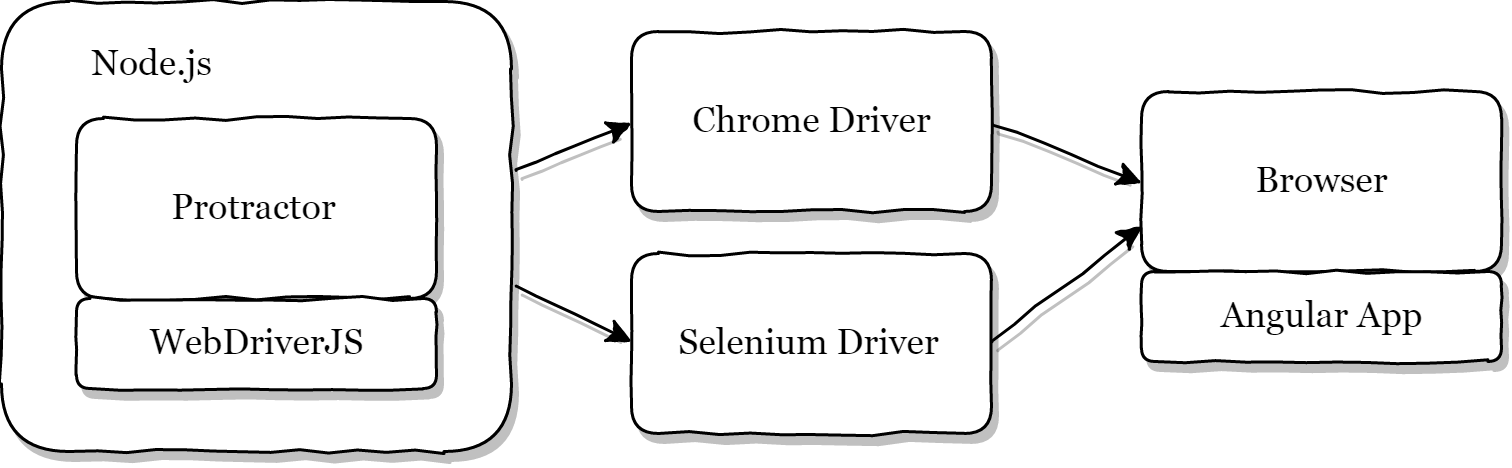
\includegraphics[width=\textwidth]{protractor}
\caption{Protractor -- zasada działania}
\label{fig:protractor}
\end{figure}

Platforma ta pozwoliła stworzyć testy automatyczne, które sprawdzają m.in. czy menu kontekstowe zawiera odpowiednie elementy zarówno w trybie widoku jak i edycji, czy poprawnie działają skróty klawiszowe, czy kliknięcie na graf w trybie edycji (i tylko w trybie edycji) utworzy nowy wierzchołek, czy graf poprawnie się eksportuje. 

Jako że Cytoscape.js korzysta z HTML5 Canvas do wyświetlania elementów grafu, sprawdzenie czy np. został dodany lub usunięty jakiś wierzchołek było nie lada wyzwaniem, ponieważ testowanie czy dane piksele mają odpowiedni kolor jest nieco kłopotliwe. W chwili obecnej udało się to osiągnąć poprzez weryfikację wyeksportowanego grafu (dzięki czemu od razu sprawdzana jest funkcjonalność eksportu). W przyszłości, gdy liczba testów wzrośnie, można rozważyć dodanie do aplikacji okna dialogowego wyświetlającego informacje o grafie -- powinno to przyspieszyć czas wykonywania się testów.

Podobnie jak testy jednostkowe, testy \textit{end-to-end} wykonują się zdalnie na serwerze Travis CI po każdorazowym wypchnięciu zmian do głównej gałęzi. Aby testy poprawnie działały na zdalnej maszynie, potrzebne było określenie konkretnego wymiaru okna przeglądarki oraz dokładnych punktów, w które ma klikać test. Było to konieczne z tego względu, ponieważ zdarzyło się, że test, który przy lokalnym uruchomieniu klikał na pustą przestrzeń, dodając przy tym nowy wierzchołek, przy uruchomieniu zdalnym trafiał w wierzchołek, zaznaczając go. 

Temat testowania \textit{end-to-end} takiej aplikacji jest ciekawy i w dalszym jej rozwoju warto, aby powstawały kolejne scenariusze testowe. Dzięki tym testom zyskujemy gwarancję, że aplikacja działa poprawnie jako całość oraz że wszystkie komponenty współpracują ze sobą tak, jak powinny. Takiej gwarancji nie mogą dać same testy jednostkowe. 

\subsection*{Testy manualne}

Aplikacja została przetestowana manualnie na laptopie pod przeglądarkami Chrome 59, Firefox 54 oraz Internet Explorer w wersji 11. Aby aplikacja poprawnie uruchomiła się pod przeglądarką Internet Explorer, konieczne było dodanie \textit{polyfilli}\footnote{Termin ten oznacza kawałek kodu, który implementuje nową funkcjonalność, która w starszych przeglądarkach internetowych nie jest dostępna.}, które w projekcie wygenerowanym przez Angular CLI nie są domyślnie importowane \cite{duveau}. Według W3Schools w chwili obecnej użycie przeglądarki IE wynosi około 4,6\% \cite{w3schools}. Gdy liczba ta będzie bliska zeru oraz gdy nowe przeglądarki będą w pełni implementować funkcjonalności uzupełniane przez ów \textit{polyfille}, wówczas będzie można je z powrotem wyłączyć (zakomentować odpowiednie linijki w pliku \texttt{polyfills.ts}). Dzięki temu wynikowy kod JavaScript zostanie pomniejszony o około 62 KB \cite{angular-browser-support}. 

Aplikacja została również sprawdzona na tablecie Lark Ultimate X4 10.1 3G IPS z systemem operacyjnym Android 6.0.0 i przeglądarką Chrome w wersji 55, który posiada 10,1 calowy ekran. Korzystanie z aplikacji na urządzeniu tego typu jest możliwe. Użytkownik jest w stanie wyświetlić graf, zmieniać ustawienie wierzchołków, dodawać nowe wierzchołki oraz krawędzie, uruchamiać algorytmy oraz wyeksportować graf. Po wstępnych testach wynika, że poprawnie działają wszystkie gesty, takie jak: przeciąganie, stuknięcie, powiększanie i oddalanie dwoma palcami czy otwieranie menu kontekstowego poprzez stuknięcie dwoma palcami. 

Jedynym mankamentem jest zaznaczanie przez pole (ang. \textit{box selection}), które na urządzeniach dotykowych możemy osiągnąć poprzez przesuwanie trzema palcami. Niestety mechanizm ten pozostawia wiele do życzenia. Na komputerze stacjonarnym czy laptopie, gdy mamy dostępną standardową klawiaturę, możemy użyć klawiszy modyfikujących (\texttt{Control}, \texttt{Shift}, \texttt{Alt}, \texttt{Command}), aby zaznaczać kilka wierzchołków oraz krawędzi. Na urządzeniu dotykowym w chwili obecnej jest to praktycznie niemożliwe i jeśli aplikacja ma być w przyszłości rozwijana, to konieczne będzie rozważenie dodania dodatkowej opcji w menu kontekstowym służącej do zmiany zaznaczenia lub przycisku przełączającego pomiędzy trybami przesuwania widoku i zaznaczania. 

Ponadto aplikacja Graphy została sprawdzona na telefonie o przekątnej ekranu 4,7 cala i rozdzielczości 540$\times$960 px. Korzystanie z niej było również możliwe i wygląda na to, że wszystkie funkcjonalności działają poprawnie. Dzięki zastosowaniu reguły \texttt{@media} z CSS3 możliwe było dostosowanie interfejsu pod tak niską rozdzielczość (główne menu jest ukrywane i wyświetlane w bocznym, rozsuwanym menu). 

\section{Przykład użycia}

W sekcji tej przedstawię, w jaki sposób użytkownik może wczytać graf, dodać do niego wierzchołek i krawędź z wagą, wykonać na grafie algorytm znajdujący najkrótszą ścieżkę, a następnie wyeksportować rezultat.

\begin{figure}[H]
\centerline{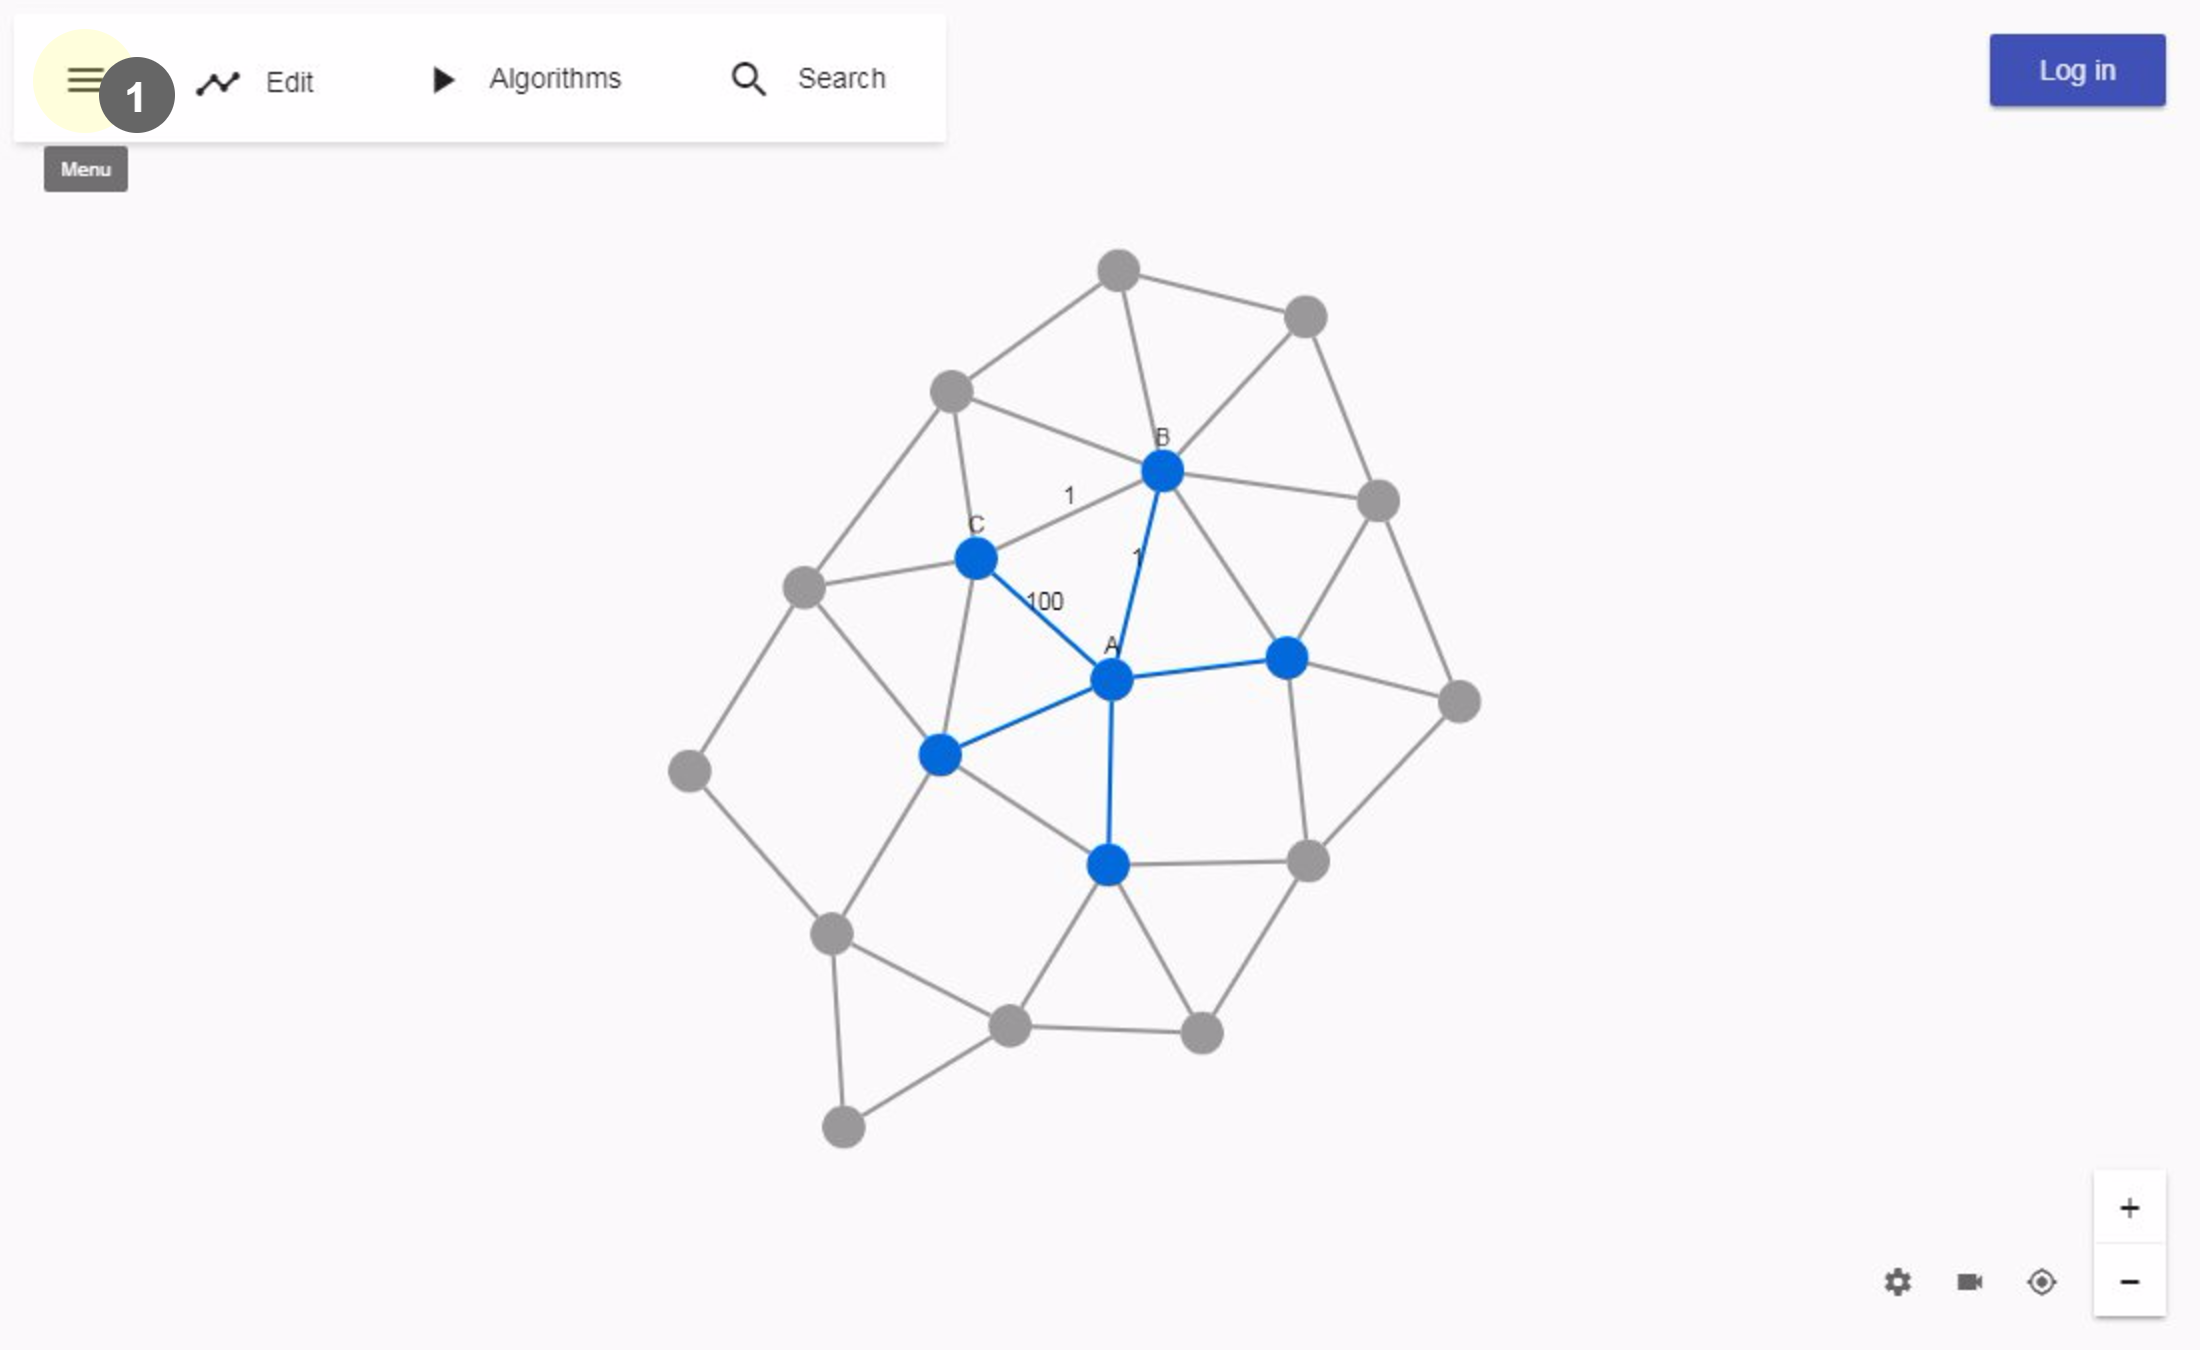
\includegraphics[width=0.8\textwidth]{use-case-1}}
\end{figure}
\begin{enumerate}
\begin{footnotesize}
\setlength{\itemsep}{0pt}
\setlength{\parskip}{0pt}
\item Otwórz boczne menu.
\end{footnotesize}
\end{enumerate}

\begin{figure}[H]
\centerline{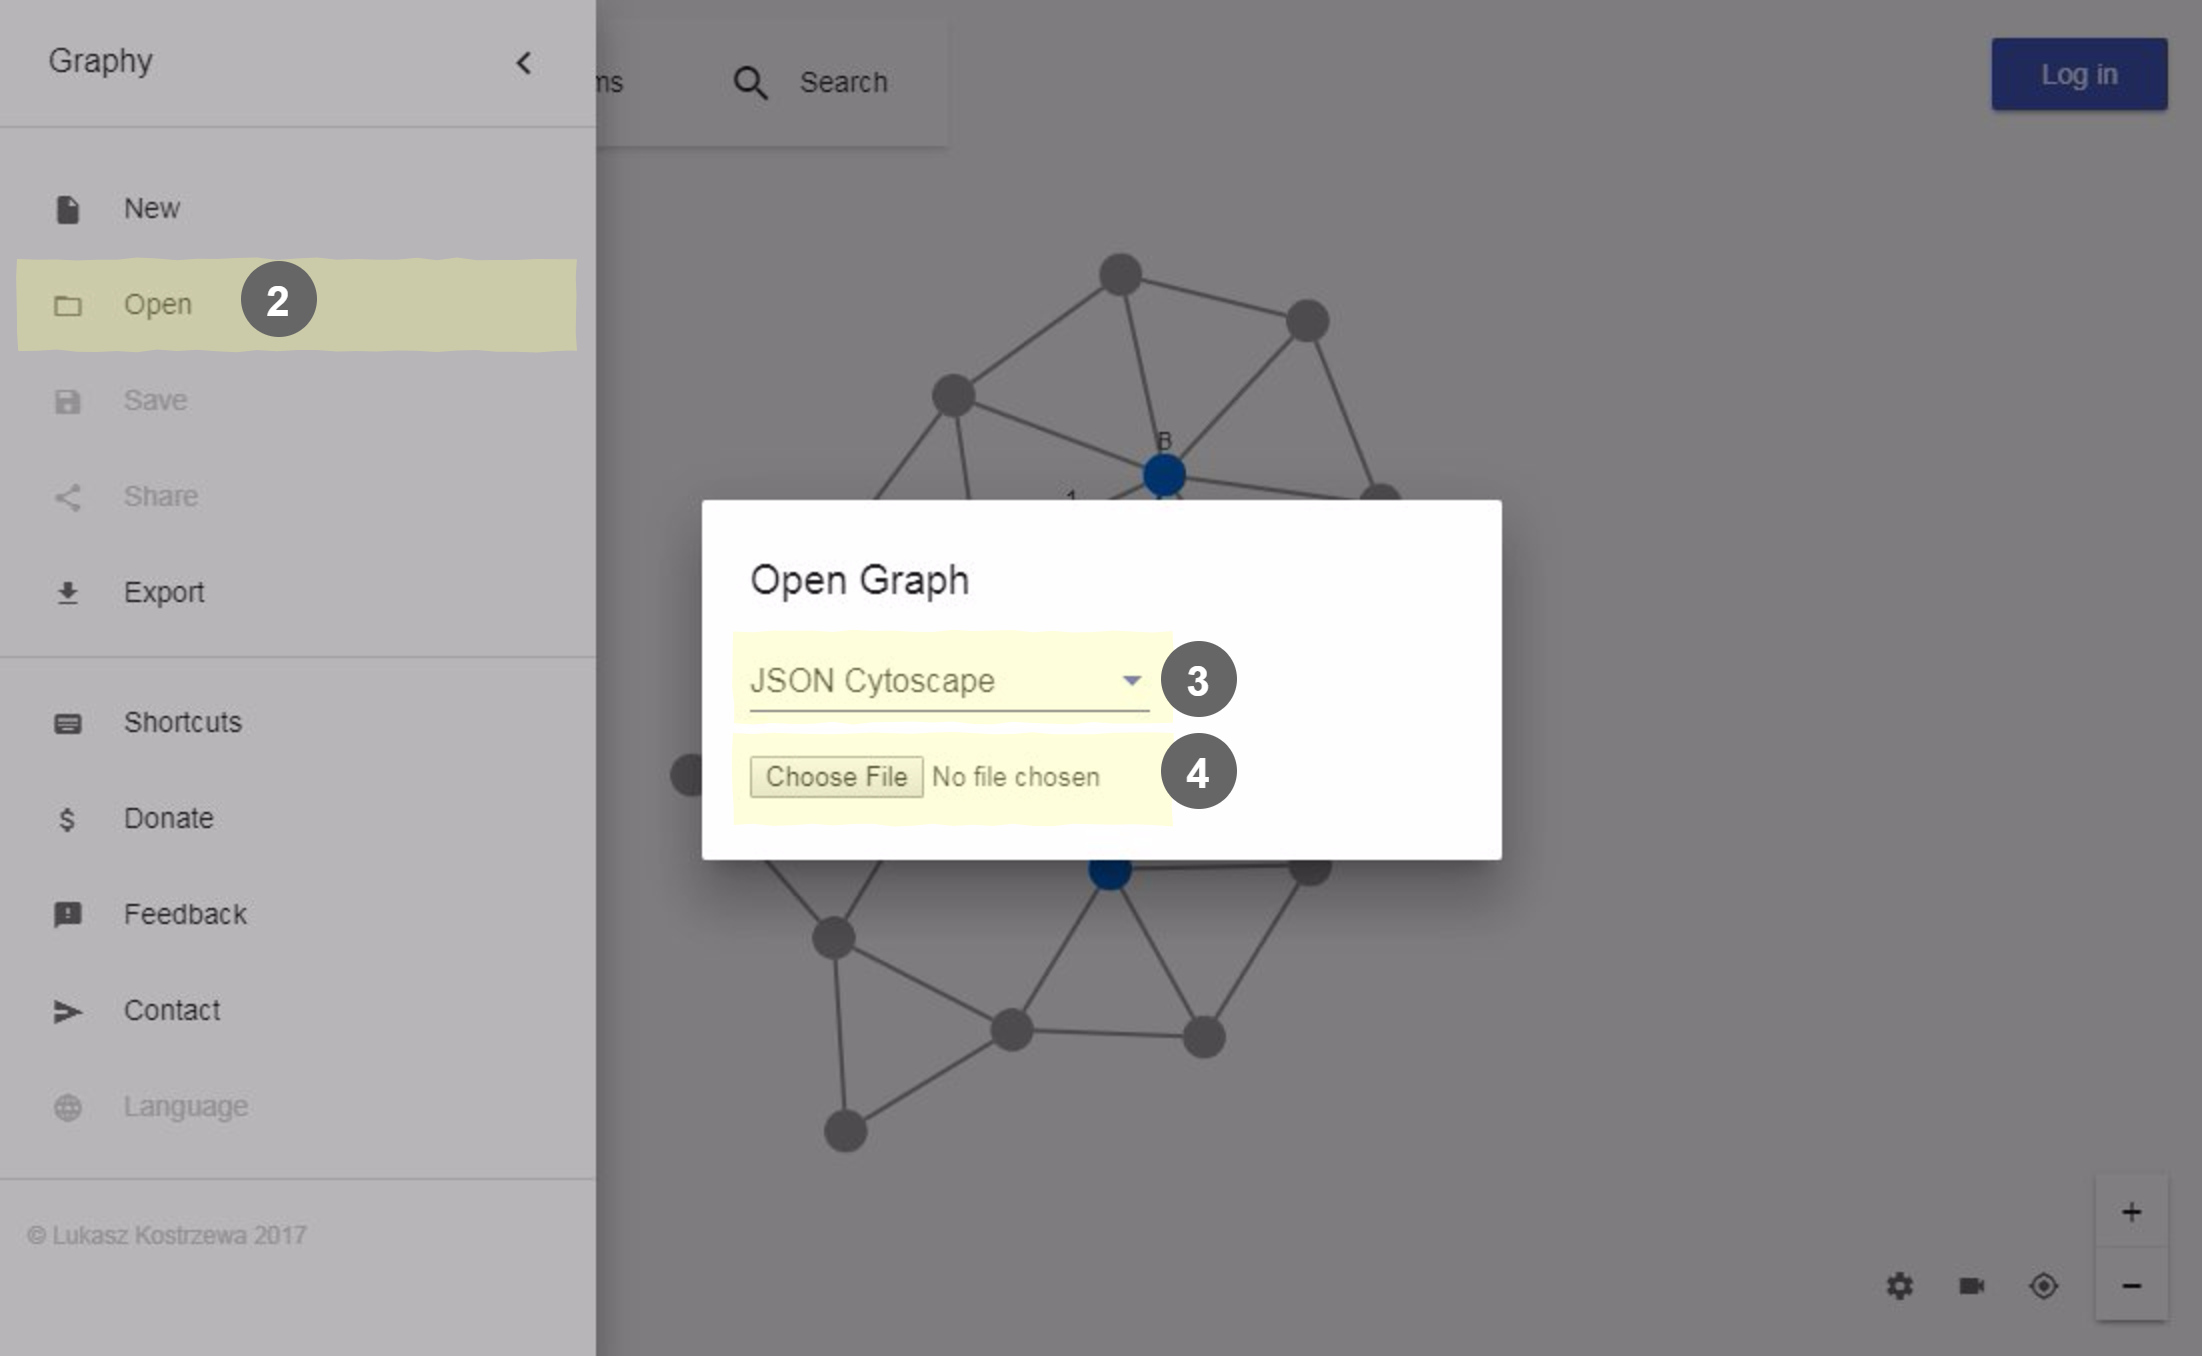
\includegraphics[width=0.8\textwidth]{use-case-2}}
\end{figure}
\begin{enumerate}
\begin{footnotesize}
\setcounter{enumi}{1}
\setlength{\itemsep}{0pt}
\setlength{\parskip}{0pt}
\item Kliknij Otwórz (ang. \textit{Open})
\item Wybierz format grafu.
\item Wybierz plik z dysku.
\end{footnotesize}
\end{enumerate}

\begin{figure}[H]
\centerline{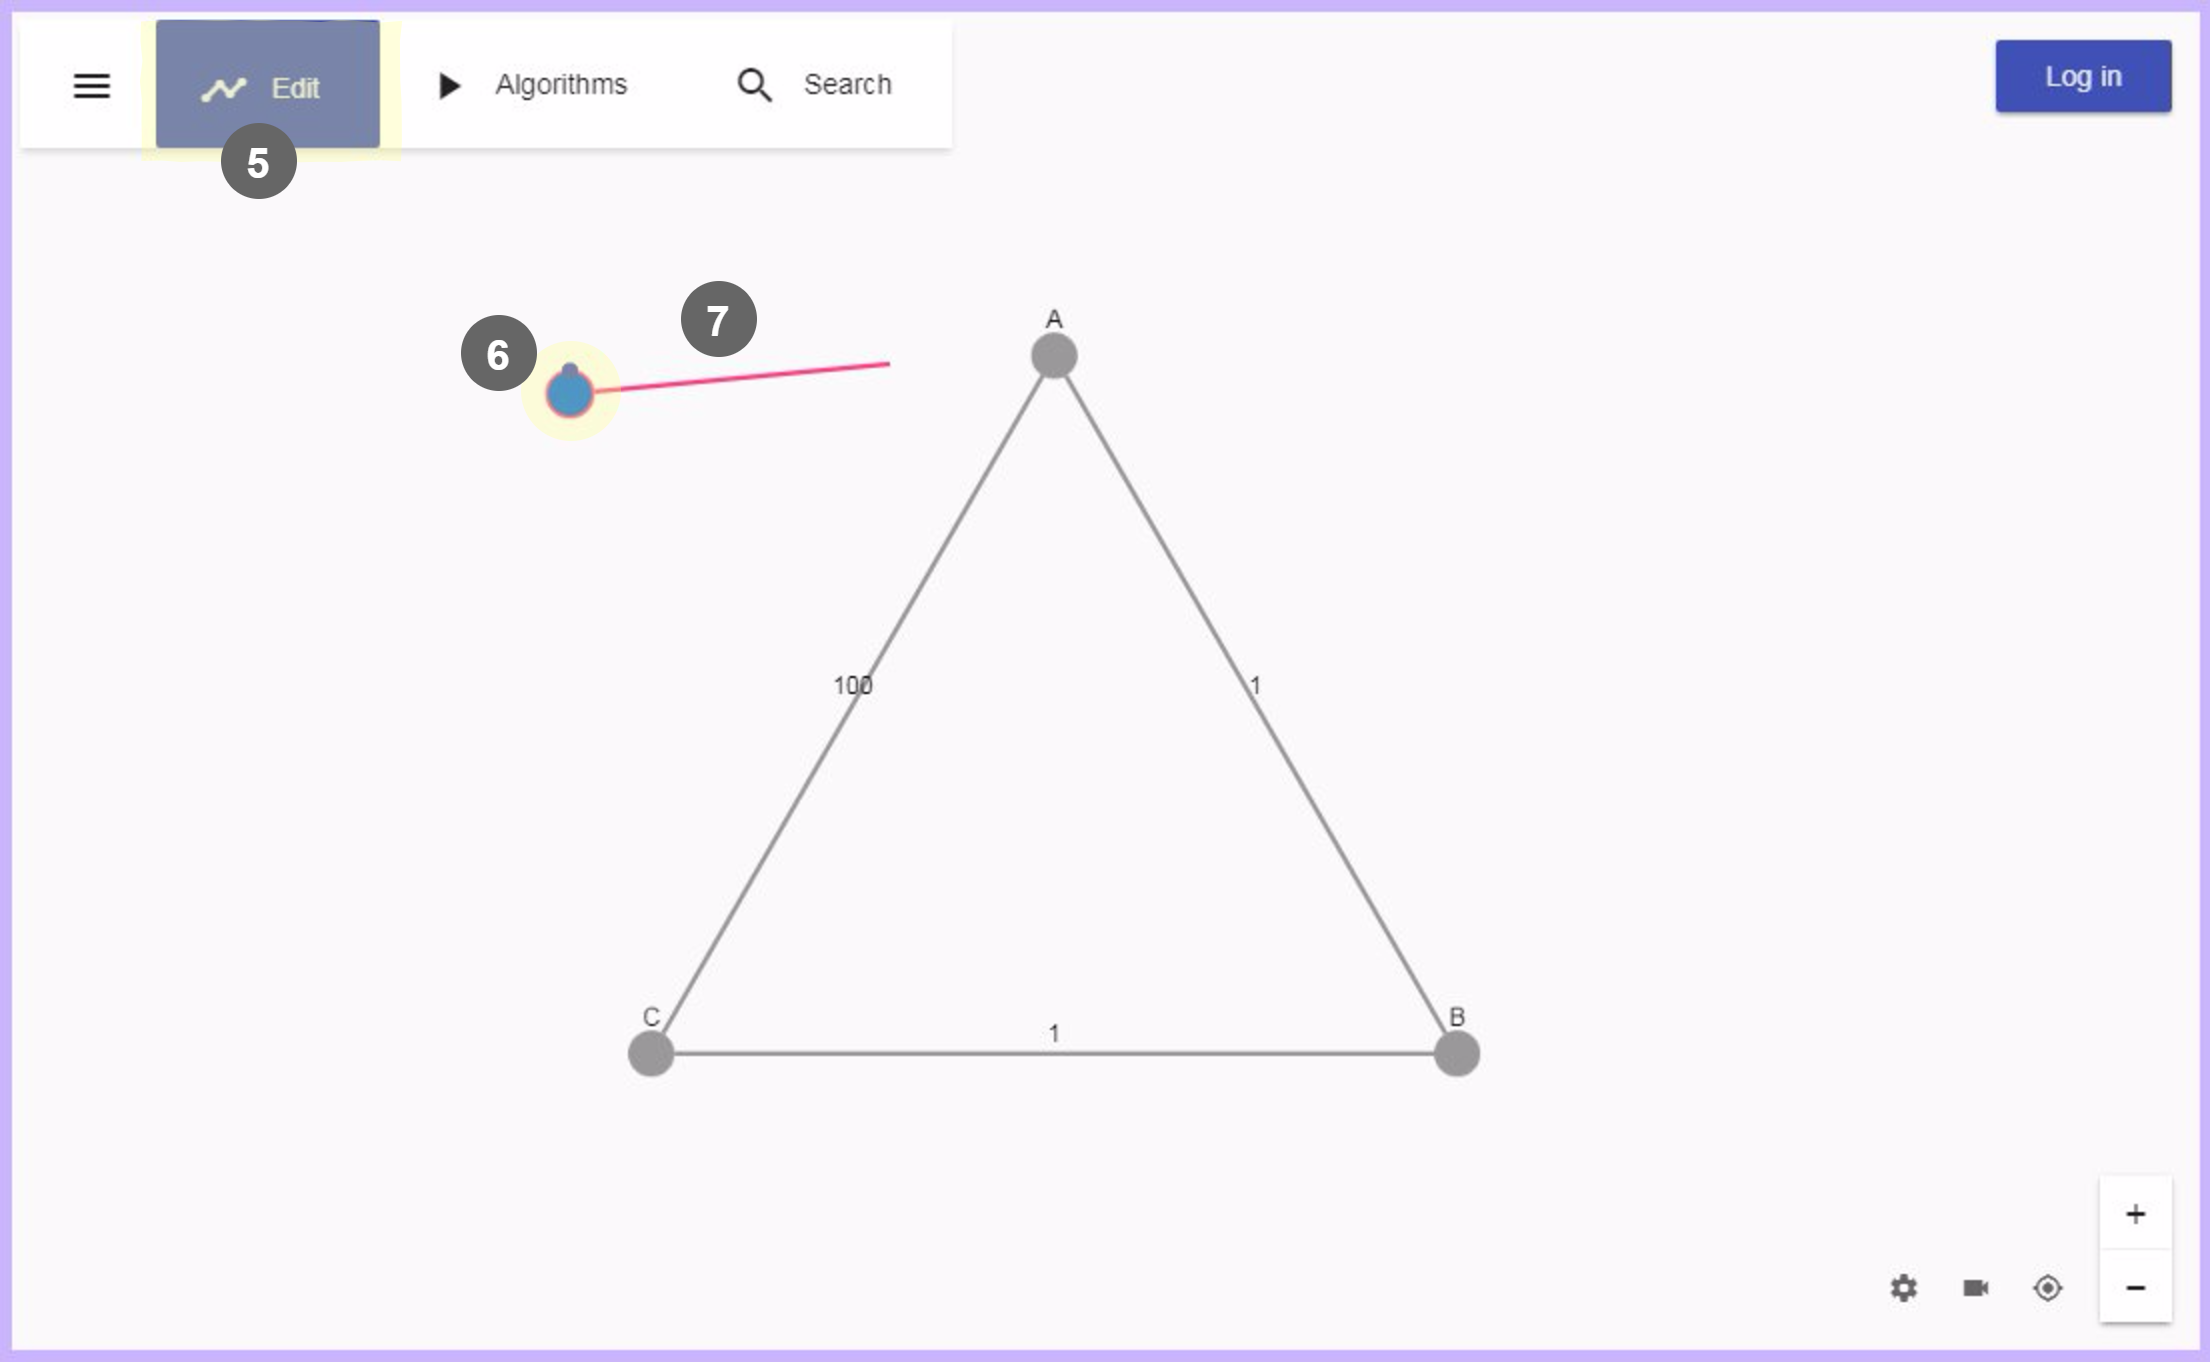
\includegraphics[width=1.0\textwidth]{use-case-3}}
\end{figure}
\begin{enumerate}
\begin{footnotesize}
\setcounter{enumi}{4}
\setlength{\itemsep}{0pt}
\setlength{\parskip}{0pt}
\item Kliknij Edycja (ang. \textit{Edit})
\item Kliknij na puste miejsce w obszarze roboczym.
\item Z nowo powstałego wierzchołka przeciągnij krawędź.
\end{footnotesize}
\end{enumerate}

\begin{figure}[H]
\centerline{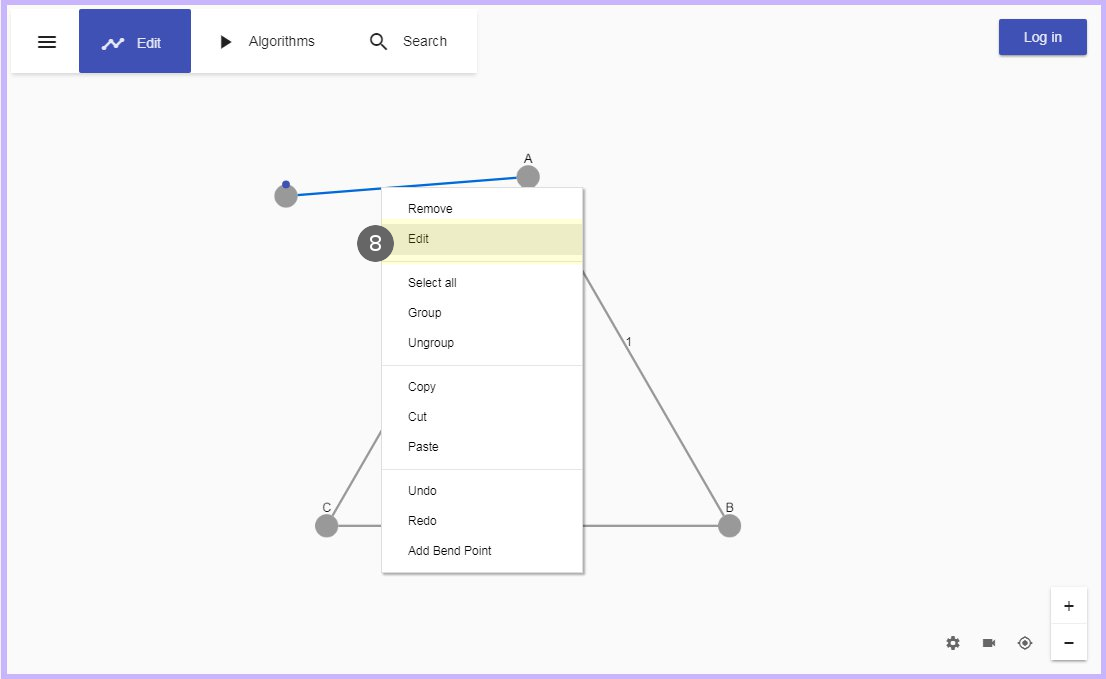
\includegraphics[width=1.0\textwidth]{use-case-4}}
\end{figure}
\begin{enumerate}
\begin{footnotesize}
\setcounter{enumi}{7}
\setlength{\itemsep}{0pt}
\setlength{\parskip}{0pt}
\item Kliknij prawym przyciskiem myszki na nowo utworzoną krawędź i wybierz Edycja. (ang. \textit{Edit})
\end{footnotesize}
\end{enumerate}

\begin{figure}[H]
\centerline{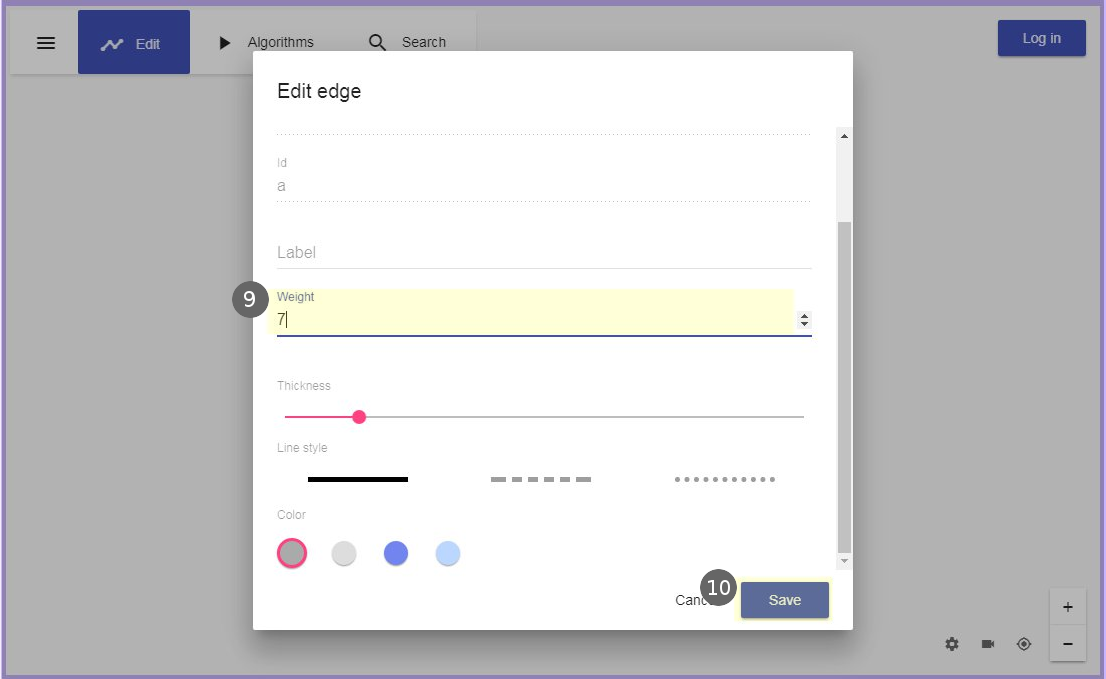
\includegraphics[width=1.0\textwidth]{use-case-5}}
\end{figure}
\begin{enumerate}
\begin{footnotesize}
\setcounter{enumi}{8}
\setlength{\itemsep}{0pt}
\setlength{\parskip}{0pt}
\item W oknie dialogowym wpisz wagę nowej krawędzi (ang. \textit{Weight}).
\item Kliknij Zapisz (ang. \textit{Save}).
\end{footnotesize}
\end{enumerate}

\begin{figure}[H]
\centerline{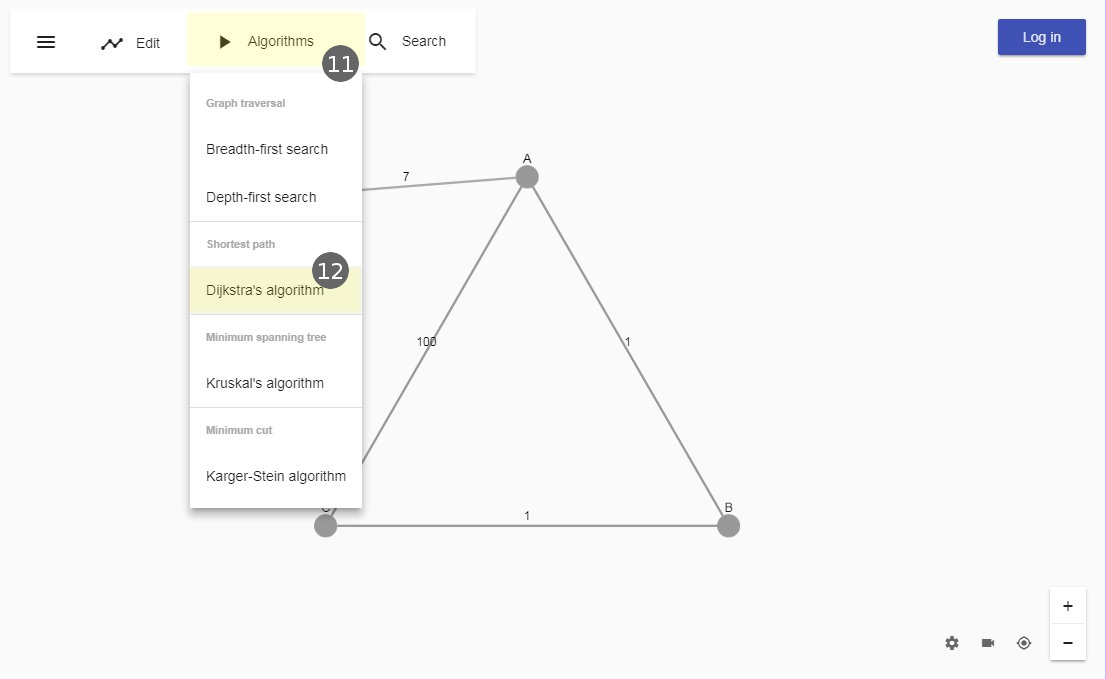
\includegraphics[width=1.0\textwidth]{use-case-6}}
\end{figure}
\begin{enumerate}
\begin{footnotesize}
\setcounter{enumi}{10}
\setlength{\itemsep}{0pt}
\setlength{\parskip}{0pt}
\item Z głównego menu kliknij Algorytmy (ang. \textit{Algorithms}).
\item Wybierz Algorytm Dijkstry (ang. \textit{Dijkstra's Algorithm}).
\end{footnotesize}
\end{enumerate}

\begin{figure}[H]
\centerline{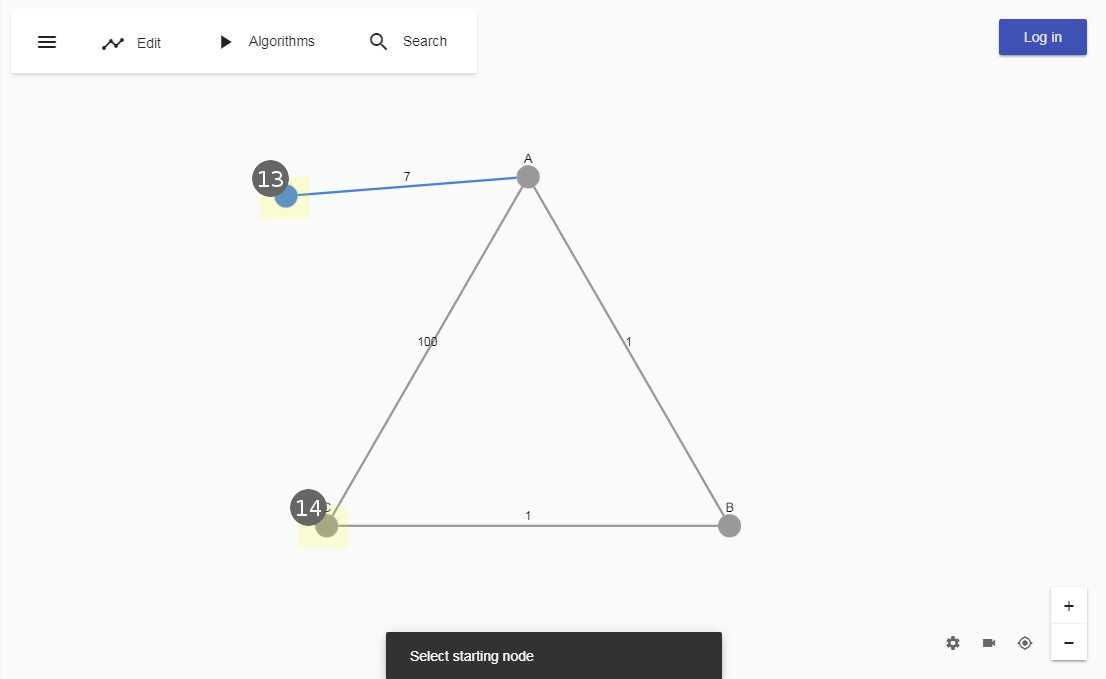
\includegraphics[width=1.0\textwidth]{use-case-7}}
\end{figure}
\begin{enumerate}
\begin{footnotesize}
\setcounter{enumi}{12}
\setlength{\itemsep}{0pt}
\setlength{\parskip}{0pt}
\item Klikając prawym klawiszem myszki wybierz wierzchołek startowy...
\item ... oraz wierzchołek końcowy.
\end{footnotesize}
\end{enumerate}

\begin{figure}[H]
\centerline{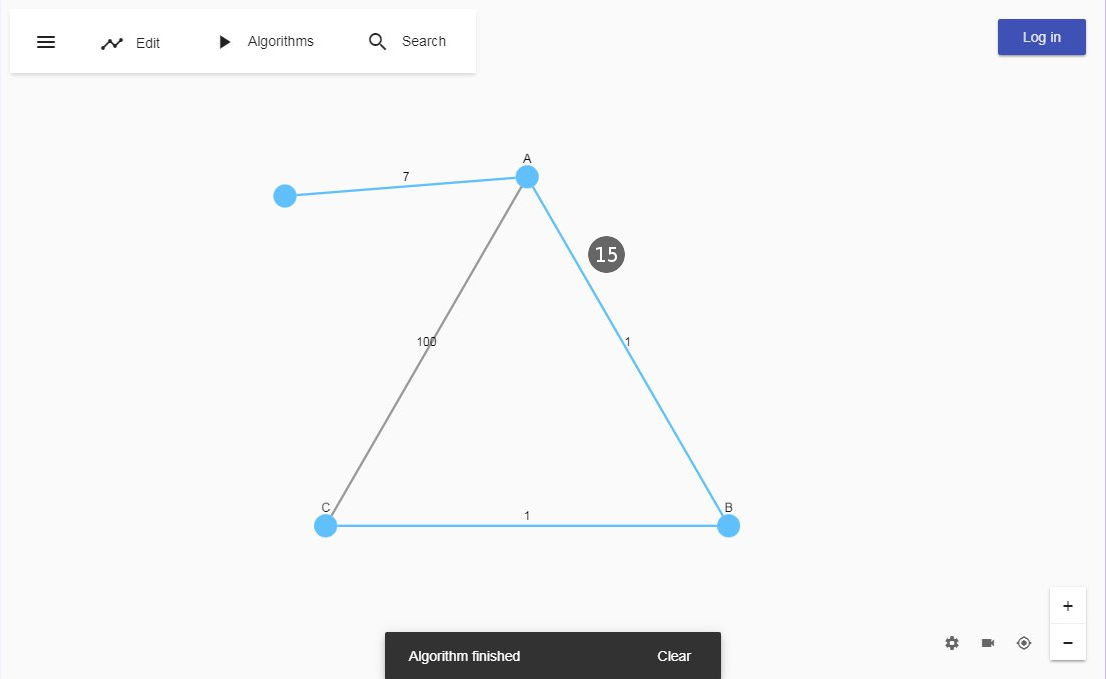
\includegraphics[width=1.0\textwidth]{use-case-8}}
\end{figure}
\begin{enumerate}
\begin{footnotesize}
\setcounter{enumi}{14}
\setlength{\itemsep}{0pt}
\setlength{\parskip}{0pt}
\item Krawędzie najkrótszej ścieżki będą po kolei oznaczane kolorem jasnoniebieskim.
\end{footnotesize}
\end{enumerate}

\begin{figure}[H]
\centerline{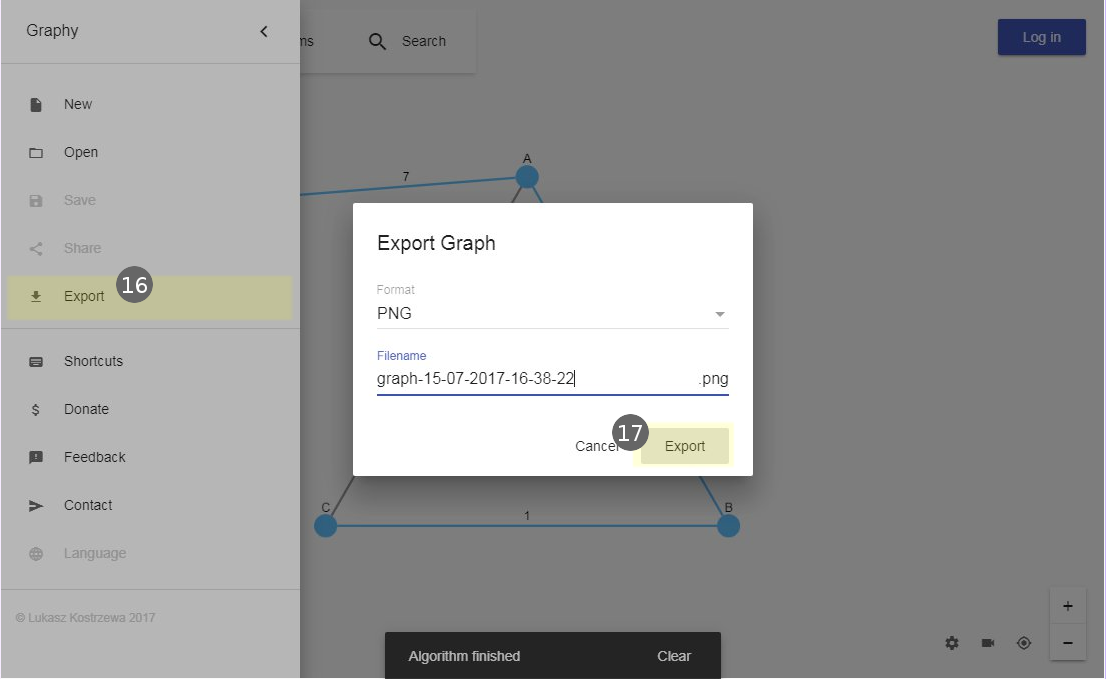
\includegraphics[width=1.0\textwidth]{use-case-9}}
\end{figure}
\begin{enumerate}
\begin{footnotesize}
\setcounter{enumi}{15}
\setlength{\itemsep}{0pt}
\setlength{\parskip}{0pt}
\item Aby wyeksportować rezultat z bocznego menu wybierz opcję Export.
\item Wybierz format (np. PNG) oraz nazwę pliku, i kliknij Export.
\end{footnotesize}
\end{enumerate}

\chapter{Instrukcje dla użytkowników}
\section{Przypadek użycia}

\chapter{Wnioski}

\clearpage
\printbibliography
\addcontentsline{toc}{chapter}{Bibliografia}

\end{document}
